\documentclass{article}
\usepackage[utf8]{inputenc}
\usepackage{amsmath}
\usepackage{graphicx}
\usepackage{float}
\usepackage{amssymb}
\usepackage{amsthm}
\usepackage[printonlyused]{acronym} 
\usepackage[acronym]{glossaries}
\usepackage{hyperref}
\usepackage[capitalise, noabbrev]{cleveref}
\makeglossaries

% \cref of cleveref: strip Eq. from equation references
% https://tex.stackexchange.com/questions/122174/how-to-strip-eq-from-cleverf
%\crefname{equation}{}{} % Completely delete Equation, even as name
\crefformat{equation}{(#2#1#3)}
\crefrangeformat{equation}{(#3#1#4) to~(#5#2#6)}
\crefmultiformat{equation}{(#2#1#3)}%
{ and~(#2#1#3)}{, (#2#1#3)}{ and~(#2#1#3)}

\title{Feedback Channels for Multicast Signals in 3GPP LTE and 5G New Radio Networks}

\author{Jonathan Smyth}
% \author[2]{\small Supervisor: Prof Sławomir Stańczak}
% % \author[2]{Bob Jones}
% \affil[1]{Department of Mathematics, University X}
% \affil[2]{Department of Biology, University Y}
% {\small Supervisor: Prof Sławomir Stańczak}
% {\small Supervisor: Prof Danielle Fontanelli}
% {\small Supervisor: Prof Dennis Wieruch}


%  keep results together, 
% keep implementation /simulations process together too. 
% highlight that this is implementation of the known tbma equations. 
% \date{Jan 2021}

\begin{document}

% \renewcommand{\maketitle}{
%   \begin{titlepage}
%   \centering
%     \begin{tabular}{lcr}
%       
\includegraphics[height=1.6cm]{uni_trento.png}
%       & \hspace{1.5cm}
%       
\includegraphics[height=1.6cm]{eit_digital.png}
%       & \hspace{1.5cm}
%       
\includegraphics[height=1.6cm]{tu_berlin.png}
%       \\
%     \end{tabular}
    
%     % middle
%     \vfill
%     {\Large	 \thetitlelabel:}\\[18pt]
%     {\Huge	 \thedegreefullUNITN}\\[22pt]
%     \vspace{5mm} %5mm vertical space
%     {\LARGE FINAL Dissertation} \\[18pt]
%     {\LARGE \thetitle}\\[18pt]
%     \vfill

    
%     \begin{tabular}{lcr}
%     \Large {Supervisor UniTrento:} & \hspace{1.5cm} &  \Large {Supervisor TUBerlin:}    \\[12pt]
%     \Large \theUNITNProf  & \hspace{1.5cm} & \Large \theTUBProf  \\[12pt]
%         & \hspace{1.5cm} &          \\[12pt]
%     \Large {Student:} & \hspace{1.5cm} &          \\[12pt]
%     \Large \theauthor  & \hspace{1.5cm} &         
%     \end{tabular}
    
%   % footer
%     % \theauthorlabel:\\
%     % {\Large \theauthor \\[6pt]}
%     % \theauthoridlabel: \theauthorid \\
%     % \theauthoremail\\[18pt]
%     % {\large \theadvisorlabel: \theadvisor\\[6pt]}
%     % \thecity, \today
%     \vspace{7mm} %5mm vertical space
%     ACADEMIC YEAR 2019/2020
% \end{titlepage}
% }
%   \centering
%     \begin{tabular}{lcr}
%       
\includegraphics[height=1.6cm]{uni_trento.png}
%       & \hspace{1.5cm}
%       
\includegraphics[height=1.6cm]{eit_digital.png}
%       & \hspace{1.5cm}
%       
\includegraphics[height=1.6cm]{tu_berlin.png}
%       \\
%     \end{tabular}
\maketitle
\newpage 
\tableofcontents
\newpage

\section*{Acknowledgements}

\newpage

\section*{Abbreviations}


\begin{acronym}[SPACEEEEEE]
    \acro{CQI}{channel quality indicator}
    \acro{i.i.d}{independent and identically distributed}
    \acro{eNB}{Evolved Node B}
    \acro{UE}{User Equipment}
    \acro{IC}{Information centric}
    \acro{FEC}{Forward error correction}
    \acro{HARQ}{Hybrid Automatic repeat request}
    \acro{PMI}{Precoding matric indicator}
    \acro{RI}{Rand indicator}
    \acro{CSI}{Channel State information}
    \acro{RNTI}{Radio network identifier}
    \acro{PUSCH}{Physical uplink shared channel}
    \acro{PUCCH}{Physical uplink control channel}
    \acro{TDMA}{Time division multiple access}
    \acro{FDMA}{Frequency division multiple access}
    \acro{OFDMA}{Orthogonal frequency division multiple access}
    \acro{CDMA}{Code division multiple access}
    \acro{EPC}{Evolved packet core}
    \acro{PMF}{Probability mass function}
    \acro{PDF}{Probability density function}
    \acro{SNR}{Signal to noise ration}
    \acro{UCI}{Uplink control information}
    \acro{DCI}{Downlink control information}
    \acro{UL-SCH}{Uplink shared channel}
    \acro{LSB}{Least significant bit}
    \acro{RRC}{Radio Resource control}
    \acro{CP}{Cyclic Prefix}
    \acro{USRP}{Universal software Radio Peripheral}
    \acro{POC}{Proof of concept}
    \acro{OTA}{Over the air}
    \acro{MAC}{multiple access channel}
    \acro{MCS}{modulation and coding scheme}
    \acro{MLE}{maximum likelihood estimation}
    \acro{MSE}{mean squared error}
    \acro{ePMF}{empirical probability mass function}
    \acro{SNR}{signal-to-noise ratio}
    \acro{TBMA}{type-based multiple access}
    \acro{crnti}{Cell-Radio Network Temporary Identifier}
    \acro{SDR}{Software Defined Radio}
\end{acronym}
\newpage

\section*{List of Symbols}

x - a scalar of dimension 1 x 1, \\
$\hat{x}$ - Estimate of value.\\
$\tilde{x}$ - \\
$\boldsymbol{x}$ - vector of size n x 1.\\ 
$\boldsymbol{X}$ - matrix of size m x n.\\ 
$|x|$ - modulus of value. \\
$\{\}$ - sets \\
$[]$ - discrete elements \\  
$\in$ - member of \\



\newpage

\section*{Abstract}
This thesis investigates an access method known as \ac{TBMA}, which has been previously researched and investigated as a suitable access method for systems which jointly wish to encode the source and channel of communication. This style of access pays particular attention groups of users who share a common goal based on a predetermined scheme. This thesis investigates and extends \ac{TBMA} in the context of LTE, investigation of \ac{TBMA} includes how we can improve the overall accuracy of the transmission. Then investigating the current state of the art for feedback mechanisms in the LTE framework, paying attention to how this can be adopted to serve a \ac{TBMA} style transmission. We then move a \ac{POC} implementation in a \ac{SDR} environment, using the open-source project srsLTE. 
\newpage

\section{Introduction}\label{intro}
\subsection{Motivation and goal of thesis}

Currently in the world there exists many different communication paradigms, most of which are content-agnostic. Which means that they take no consideration into the actual meaning behind the data, ignoring any potential patterns or commonalities. Their primary concern is to transfer arbitrary data from A to B. We read "this dichotomy of information content and significance has been a conceptual advance in classical data communication targeting reliable high-speed data transmission" in \cite{kountouris}. 
However, as the world is becoming more connected, such areas as Industry 4.0, immersive video/audio and Internet of things begin to prompt more questions about the issues surrounding massive networks and their access methods. As these content-agnostic methods offer the possibility to retrieve granular user specific payloads, which requires resource scaling linearly to the number of users in the network \cite{aloha,graphbased_analysis,coded_ran,capacity_gauss}. In contrast to the aforementioned approach, new communication paradigms are emerging, one such approach would be information-centric. Information centric  medium access protocols are designed to recover information of interest rather than the specific payloads \cite{kountouris,sem_coms,sem_filter,source_chane_coding,source_chane_coding2}. \ac{IC} communication moves away from traditional methods by making the main objective of the protocol a shared goal, rather than just a means of transmitting data. The goal-oriented approach utilises the shared objective of the users signal reconstruction at a fusion centre. 

If we consider applications like inner city autonomous driving in an LTE context, these users are highly dependent on a reliable and efficient communication link between infrastructure and other connected users. Thus they need to be able to feedback \ac{CQI} to an intended receiver (e.g a base station). Normally this is completed with a dedicated resource and the base station disregards any statistical correlation on multiple users transmitting this \ac{CQI} information. However, in reality in a busy city, the base station would actual want to aggregate all this information form multiple groups of autonomous vehicles to best understand what the real world environment is currently like, thus being able to efficiently coordinate its resource available and best serve the entities in their respective cell-region or groups. However, current methods of broadcast/multicast offer communications without link quality information to the target group. Feedback mechanisms are generally present only for unicast transmissions. With the current implementation in the LTE framework, multicast feedback mechanisms could only be achieved through unicast feedback.

In order to enable efficient feedback mechanisms for multicast communications, information centric communication approaches, e.g. based on type based multiple access (TBMA)\cite{tbma}, promise an efficient implementation. This is further justified if a large number of devices with strict latency requirements are taken into account, rendering dedicated feedback channels ineffective. 

In this thesis, an information centric feedback mechanism for multicast signals shall be investigated. The information centric access method, \ac{TBMA}  will be investigated through literature and simulated to find key parameters which improve the robustness of transmission, different styles of encoding the channel will be investigated. 
Current LTE Feedback mechanisms shall be first investigated through literature, to understand how they work in the current setup and point out and potential areas in which they could be applied to the context of this thesis. Next using a SDR project, "srsLTE" a proof of concept implementation of the above investigation about both \ac{TBMA} and Feedback mechanisms will be conjoined to produce a proof of concept implementation for LTE feedback over TBMA for multiple users. 


\subsection{Problem and Context}\label{prob_context}
%  extension of the bullets points etc 
%  can use bullet points here , really just point out which problems i am approaching.
In classical device centric communication, the source and the channel are encoded separately, thus the channel is independent of the data \cite{shannon_theory}. Many different approaches exist for the classical device centric communication approach, CDMA, TDMA and FDMA \cite{multiple_access_protocols}.  However information centric communication (ICC) approaches the problem differently, by jointly encoding both the the source and the channel. ICC utilises the knowledge of both, source  and channel coding, which means that prior to transmitting the information, all parties involved in the ICC transmission are aware of how the channel is encoded and what the encoding scheme means~\cite{information_centric}. The following list outlines some of the major problems at the time of writing this thesis. The purpose of this thesis is to address these problems and propose a suitable solution with a \ac{POC}  

\begin{itemize}
  \item Each feedback message consumes one resource, and scales linearly with each user, this is inefficient due to the increasing number of connected devices. We discuss this issue in \cref{intro}.
  \item As more users/devices become connected, more problems arise about how to access the medium efficiently. Conventional access methods become redundant, see \cref{intro}
  \item Current methodologies do not consider potential relationships in the data being transmitted. Situations arise in the real world where, for example multiple users in a group would like to transmit an ACK/NACK bit in response to a group message, currently each user would require a dedicated resource and its associated resource costs to achieve this. TBMA would offer a less resource intensive approach \cref{intro}. 
  \item Feedback mechanisms such as CQI and ACK/NACK which are crucial for the link adaption to ensure most efficient use of available resources. Currently these mechanisms are only supported for unicast in LTE. 
  \item The LTE framework currently offers feedback options as discussed in \cref{sota}. However, no option really for multicast feedback, other than using unicast feedback.
\end{itemize}

First we should outline that, more traditional access methods are in place to differentiate between when and how user are transmitting information and avoiding interference between different transmissions. If we consider two situations in wireless communication when multiple users are transmitting information simultaneously, interference can occur. If we consider when two waves come close to one and other, their effects in essence add together, depending on the waves phase, dictates whether this is constructive or destructive. Constructive interference occurs when the maxima of the waves are in phase, such that the amplitude of the resulting wave is equal to the sum of the individual amplitudes. Conversely when the maxima of the waves are 180 degrees out of phase, the resultant amplitude of the waves is 0, thus in effect these waves cancel each other out. 
% The affects of being in or out of phase can be viewed in \cref{fig:wave_inter}. 

In the context of multicast feedback, which inherently is more than one user responding to a group transmission this can be a problem in transmitting the feedback information as undesirable destructive interference can result in the final waveform received at the eNB being unusable due to the combining waves destroying each other. Conversely, the interference can also play in the favour of the feedback, waves in phase would have an additive nature on the final reading at the eNB. 


% \begin{figure}[H]
%     \centering
%     \includegraphics[
%       width=6cm,
%      height=7cm,
%     keepaspectratio,]
%     {interence_waves.png}
%     \caption{Constructive and Destructive wave interference \cite{interference_pic} }
%     \label{fig:wave_inter}
% \end{figure}

% problem statement we want to find the true distribution etc. 

Consider two similar scenarios in a multicast transmission from a base station, the base station transmits some information to all its grouped users. First the eNB wants feedback information about, for example, the quality of the downlink channel . As TBMA is information centric, each encoded subcarrier on transmission has a particular non arbitrary meaning, which in the case of device-centric may not be true. As we jointly encode the source and the channel, potential interference should be mitigated which could be introduced in device-centric approaches. Second, the base station instead of feedback information, wants normal uplink traffic, which could be any kind of arbitrary data from a user, in this case, more conventional device-centric approaches may be of better use. In this thesis we show that significant gains can be realised in estimation quality and in system resource consumption if the physical layer and the multiple access are designed jointly for the purpose of estimation, not just explicit value retrieval.

Using information centric approaches such as TBMA, would allow simultaneous usage of the resources available and substantially reduce the latency of the feedback. Users in a massive sensor network would allow for different types of information to be fed back to the base station. In LTE different modulation schemes exist which are used depending on the quality of the wireless channel. Modulations scheme play a key role in adapting to noisy environments and allow for consistent and efficient transmission of data. One such indicator which plays a role in the type of modulation used in data transmission is the \ac{CQI}. Consider the scenario when multiple users receiving unicast transmissions, each UE, could be anywhere in the cell region with unknown obstacles or interference, this means that there exists the situation when different modulation schemes are being used for different UEs attached to the base station. 

In the case of multicast user groups, it is not possible to modulate a single multi cast in different schemes, instead a single scheme is needed for a single multicast to many users, this scenario in itself elicits the same logically inefficient error we see in the aforementioned paragraph as all users in the group would need to relay their own \ac{CQI}. Instead, a better approach to understand the collective consensus of the \ac{CQI} and thus deriving the bare minimum modulation needed for a sufficient transmission would be via a TBMA approach where each user constructs a PMF of their \ac{CQI} history for a given time period, this would allow the eNB to better and more efficiently adapt their multicast transmission to best suit the users. If we look at \cref{fig:pmf_subcarriers}, we can see that how we could understand a collective TBMA transmission, with the source and channel encoded with a particular goal in mind. This example of an CQI transmission could be exactly what is needed for a base station to understand an overall idea of how the multicast channel is performing. Thus choosing an appropriate modulation scheme which would suit the masses. 

\begin{figure}
    \centering
    \includegraphics[
      width=8cm,
     height=12cm,
    keepaspectratio,]{cqip_subcarrier.png}
    \caption{PMF of all users results of feedback across available subcarriers.}
    \label{fig:pmf_subcarriers}
\end{figure}

Given the above example, we can see how it is no longer important to understand what every individuals exact measurement is, rather it is more important to get an overall understanding of how good the channel quality is for the majority of the users in a group. Under this premise, we do not need to know that i.e exactly 15 UEs had a CQI of 6 and 8 UEs had a CQI of 12. In this situation the granularity of the data is less important. Knowing this information can allow sensible choices of modulation schemes by the base stations and better use of radio resources as an overall, whilst satisfying the overall needs of a group instead of the individualistic. 


\subsection{Thesis Structure }
% add some information to the abstract for what exactly has been done. 
% finally the to comes to a 3-5 bullets on what has been done. cite the johannes 
% my part is really on how to implement this on LTE..
% maybe have some contributions part here?? 
%  exact contribution on what is the aim. and the outcomes of thesis. 
%% overall general structure of the thesis and what to expect.
% specific research question...conceptualise the application of both parts to LTE framework. Make a specific list of 
The thesis is structured as follows; firstly a short introduction will be given in \cref{intro}, next the problem we are facing and context of why this approach is ideal in \cref{prob_context}. With some background motivation understood, we would move onto the current state of the art approaches for feedback in LTE and multiple access methodologies which is found in \cref{sota}, this section presents also the current process in the LTE framework of how feedback mechanism work. Next, we would move then into the \cref{tbma_sec} where the system model for TBMA is presented and discussed. This will give the basis of the mathematical model which is to be understood for TBMA. Data specific models are then presented in \cref{data_models} based on potential use-cases for TBMA, this will illustrate how TBMA could be applied to different data models in the real world. Once the model is understood, the process of how we can estimate the parameters based on our model is then presented in \cref{param_estimation} and discussed, this is broken down based on a random complex channel and an identical channel \cite{tbma}. After we set our theoretic framework, some examples of real world applications of TBMA are presented in an illustrative and informative manner, showing how the different subcarriers and channel structure should look, see \cref{schemas_and_channels}

Next, we would move on to the simulations and numerical analysis of the results of TBMA, comparing different features of the channel architecture that we can exploit to tune our results and optimise the channel, see \cref{sim_results}. Next a discussion on the application to the LTE network in depth and how thee feedback could be achieved given the current LTE implementation, this is discussed and presented \cref{lte_app}. A proof of concept implementation based on the open source project srsLTE is presented and tested in a more realistic environment than the simulation in \cref{srslte_poc}. Finally, future steps and outlook of TBMA are presented in \cref{summary_out}. 





\section{State of the art} \label{sota}
This section gives an overview of the current state of the art approaches for multiple access methodologies, moving onto one of the main themes of the thesis, Type Based Multiple Access (TBMA). TBMA is presented in its generic context as a multiple access method, the system model is then presented and discussed with a generic data model, this underlying information gives the basis to move onto more application specific use-cases of TBMA. 
The section then moves onto an investigation into which feedback mechanisms are available in the LTE network, how they work from an architectural point of view, what each of the metrics are used for and how the encoding process should look like in the wild.

\subsection{Multiple Access}

In general within wireless communication systems, multiple devices share the respective "wireless resources". In order to coordinate this situation, we need to have an access scheme which describes how the resources are shared and then also an access protocol which defines how the devices access the the resources, i.e scheduled,random or contention etc. A radio resource can be thought of as a proportion (this can be multiplexed by time, frequency or code) of the wireless radio medium which is available \cite{access_tech}. Although this thesis is not interested explicitly in traditional multiple access methodologies, some background on how they function is a good basis to understand and highlight the utility of TBMA in the thesis's context. The comparative overview of traditional access and what could be referred to "new age" access will highlight why TBMA is sensible for the context of this thesis. 

\subsubsection{Access Technologies}
Currently there exists three primary methods of multiple access (there are many variations on these). Time-division, Frequency-division, Code-division. The following points outline the basic methodology behind these access technologies, paying attention to how they access the medium. TDMA - Time Division multiple access,  relies on signals which have been digitised and is based on time division multiplexing \cite{tdma_info}. TDMA in essence allocates different time slots for the users of a channel to transmit their data. In TDMA systems, the spectrum of the available radio is divided into user specific time slots, only the allocated user can transmit on that respective slot \cite{tdma_info}.
CDMA - Code division multiple access uses spread spectrum techniques, meaning each user is not allocated a particular frequency, instead they utilise the full available spectrum. CDMA transmissions are encoded with pseudo-random digital sequences, which are separated by orthogonal codes\cite{cdma_info}. The receiver knows the user specific code sequence and uses said sequence to decode the received signal, this is possible because the cross correlation between different users is small. This can be achieved as the bandwidth of the code signal is chosen to be vastly larger than the information signal, the encoding spreads the signal across the entire spectrum \cite{cdma_info}.
FDMA - Frequency division multiple access (FDMA) assigns users an individual frequency band of the entire available wireless channel frequency. Each users' channel is allocated on demand when entering the cell region \cite[Section...]{fdma_info}. All active adjacent frequencies in a cell are divided by a guard band to reduce cross talk between channels. FDMA is based on frequency division multiplexing and each user has a separate frequency for both uplink and downlink \cite{fdma_info}. OFDMA - Orthogonal frequency division multiple access (OFDMA) is the multi user variant of orthogonal frequency division multiplexing (OFDM), where multiple access is achieved by assigning different sub carriers to different users. This approach allows simultaneous data transmission from several users. The OFDMA approach means the radio resource is two-dimensional (2D), contiguous or non contiguous sub carriers span the frequency and at the same time an integer number of OFDM symbols span the time domain\cite{ofdma_info}.

Clearly from the above definitions it can be seen that these approached do not take any consideration into the actual payloads of the transmission, these approaches offer a means to transmit any kind of data through a medium based on the predefined protocol. The above approaches are ideal when the there is no prior knowledge about the information being sent.

\subsubsection{Type Based Multiple Access}

Communication channels need to be designed to meet certain requirements and with the ability to handle many users or increased efficiency of limited resources. Firstly, looking at multiple access method for the wireless channel which are device-centric approaches, where device-centric could be described as "A device is often viewed as having a function independent of the environment in which it might be used. The view caters to the intended function, tends only to mention a device’s properties or behaviour, and assumes an intended environment: it is “device-centric”." \cite{device-centric}.

On that definition it can be said that the device-centric access assumes no real interest in the actual payload being sent, rather just that arbitrary information needs to get from A to B. We can see that in this ubiquitous "one size fits all" approach that there could be redundancies when similar goal-orientated information is to be transmitted. Thus potentially leading to bottlenecks in busy networks due to the overhead needed to serve arbitrary information. 

% instance of information centric protocols 
%  multiple devices share the same resources, based on this type based .
Information centric access differs from device centric in the sense that we wish to access a channel through information type apposed to device type. As in device type we are not worried about the payload rather the device transmitting it, information centric is positioned to access based on the type of information being transmitted regardless of whom it has come from \cite{information_centric}.

With the understanding of what device-centric communication is and how it is "scheduled" or "random", we can see that indeed when there is a common goal in transmission and not just arbitrary communication, that the problems discussed in previous sections could be mitigated when we jointly encode the source and channel. This joint encoding is achieved through \ac{TBMA}. 

In this section we will discuss a multiple access method known as Type Based Multiple Access (TBMA). This is a new approach for users to gain access to a channel. We will discuss TBMA explaining the approach and looking into the generic system model and how it works with a generic data example. 
TBMA - Type Based Multiple Access, TBMA is also an orthogonal access scheme, however there is one key difference between TBMA and the aforementioned access schemes. TBMA is an information centric approach, meaning that the source and channel are jointly encoded for transmission. In information centric communication, the users have prior knowledge of how the the channel is to be encoded and how the source is to be encoded. This means that for example, all the users in a TBMA transmission are not as flexible to send arbitrary information as the aforementioned counterparts, however this is not the goal of TBMA. TBMA is a method to be used when there are commonalities in the transmissions or when the data to be transmitted amongst all the users of TBMA is sharing some similar goal. Conversely this differs greatly to the arbitrary source encoding which occurs in the likes of TDMA,CDMA and OFDMA etc. it could be said that these approaches are device centric meaning the source is not jointly encoded. 

We will present and discuss the system model for TBMA. To begin, we should first look from a high level what exactly is happening. In device-centric systems, the channel is designed to handle data transfer regardless of the source it has come from. Likewise, the source is designed irrespective of how the channel looks. device-centric approaches may be beneficial for arbitrary data when the information of each specific device is of interest. However, in the case of TBMA, we may not actually be interested in the specific information each user has, rather combined information that can yield metric of interest, such as \ac{PMF}. 

In general terms in TBMA, if we consider that a group of sensors $k$, observes conditionally \ac{i.i.d} data $X_1 \dots X_k $ given a parameter $\theta$. For conveniences sake, it is assumed that each $X_k \in \{1 \dots R\}$ takes on a discrete value (where $R$ is the total number of potential outcomes in the specific use case), with a \ac{PMF}~${p_{\theta} = [p_{\theta}(1), \ldots, p_{\theta}(R)]}$. The \ac{PMF} belongs to a family $\{p_{\theta}: \theta \in \Theta\}$ where $\Theta \subset \mathbb{R}$ is the parameter space.. Each sensor node in the group then transmits a waveform $s_{k,X_k}$, which is constructed based on the sensor nodes index and the observation of that sensor node, $X_k$. To access the wireless channel, each sensor transmits a signature waveform $\boldsymbol{s} \in \mathbb{C}^{N \times 1}$ selected from the orthonormal signature matrix $\boldsymbol{S} \in \mathbb{C}^{N \times R}$. This matrix contains all possible outcomes of the available observations and acts as a key for the user when they observe their observation

There exists an energy constraint that must be satisfied such that \textbf{ $||\textbf{s}_{k}^2|| \leq E$}, which means that the transmission of each node must not exceed the limit of the total energy available for the transmission. The transmitted waveforms are received through a Gaussian multi access channel. The fusion centre then produces and estimate of the $\hat{\theta}$. The over all objective thus of the TBMA is to design the channel waveforms and estimator such that the error of the ground truth and received signal is minimised (a suitable method could be using the mean squared error)\cite{tbma}. A graphical representation of the above notation and design has been shown in \cref{fig:tbma_general}. 

\begin{figure}[H]
    \centering
    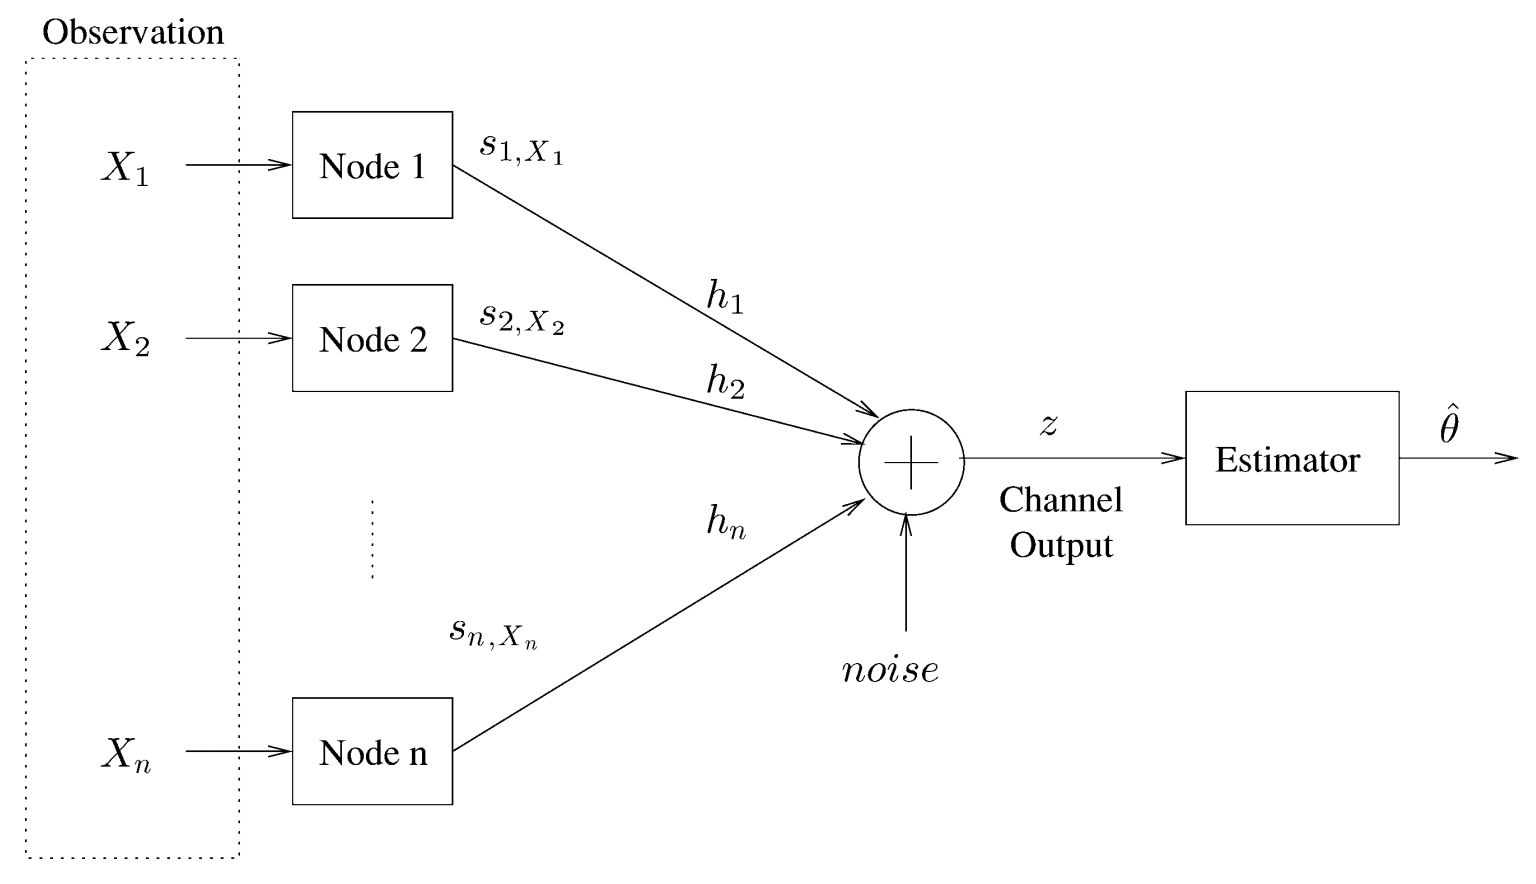
\includegraphics[
      width=10cm,
     height=10cm,
    keepaspectratio,]{tbma_estimation.png}
    \caption{TBMA Estimation over Multi Access Channel}
    \label{fig:tbma_general}
\end{figure}

Now we should present and discuss the system model for TBMA. As we have set the scene is the previous paragraph about how the different aspects of the systems model come together. In waveform design, a crucial observation is that the estimator doesn't actually need to know the exact values of $X_1 \dots X_k $, to achieve its best performance \cite{tbma}. In reality, if each of these nodes could deliver a sufficient statistic with their respective transmissions, then there is actually no loss of information. An example of such a statistic would be the empirical measure , i.e the type:
% define emperical measure . define it in words...
\begin{align}
    \tilde{p} = \frac{1}{k} (N_1 ,\dots, N_R),
\end{align}
where $N_j =\sum_{k=1}^K 1(X_k = j)$ is the number of sensor nodes in the network that observe $j^4$. If we let $u_1,\dots,u_R$ be $R$ orthonormal waveforms, and then setting;

\begin{align}
    s_{k,X_k} = \sqrt{E}u_{X_k}, 
\end{align}

which corresponds to letting every node observing $j$ transmit $u_j$ with energy $E$. With $h_k$, is the channel response, which is assumed to be constant during the $k$-th transmission.  We then arrive at the signal at the fusion centre which is presented as:
%  watch out for inconsistency in the terms in the equatsions 
\begin{align}
    \boldsymbol{y} = \sum_{k=1}^K h_k  \sqrt{E}u_{X_k} + \boldsymbol{w}, \label{eq:system_model}
\end{align}

Where $\boldsymbol{w}$ is the channel noise, which is assumed to be white proper-complex Gaussian noise $\mathcal{CN}(0, \sigma^2 \boldsymbol{I}_N)$ and with power $\sigma^2/2$.  This becomes easier to understand when we consider an identical channel, where all $h_k$ terms are considered as equal to 1. Which then would be simplified to;

\begin{align}
    \boldsymbol{y} = \sum_{j=1}^R \sqrt{E}N_j u_{j} + \boldsymbol{w}, \label{eq:simplified_system_model}
\end{align}

% \begin{align}
%     \boldsymbol{z}^l &\triangleq \left[\langle \boldsymbol{y}^l, \boldsymbol{s}_1\rangle, \ldots, \langle \boldsymbol{y}^l, \boldsymbol{s}_R\rangle  \right]^T, \label{eq:mf_output}
% \end{align}

We see that the received signal contains a noisy version of the empirical measure once we have applied a matched filter of $u_1,\dots,u_R$ and scaled by $1\sqrt{E}k$, we arrive at;

%
% after matching filtering here. 
\begin{align}
    \boldsymbol{z} &= K \tilde{\boldsymbol{p}} + \boldsymbol{w}, 
    \label{simple_estimation_indentical}
\end{align}

Therefore in the case of this deterministic channel, the estimate can directly obtain as:
%
\begin{align}
    \boldsymbol{\hat{p}} &\approx \boldsymbol{z} / K. \label{eq:est_const_sys}
\end{align}

Given the above estimation method, we observe some notable pieces of information, for $K \rightarrow \infty$: The estimate \cref{eq:est_const_sys} converges to the true PMF in the region of high SNR values where the noise is playing less of an influential role on the measurement, i.e.~$D(\hat{p}\| p_{\theta}) \rightarrow 0$, where $D(\hat{p}\| p_{\theta})$ is defined as the distance between the original distribution and the distribution of the output of the channel, such metrics could be \ac{MSE}. 
Conversely, with low SNR values, we can improve the estimator can be by averaging over multiple observation times $l$, where the user $k$ re-transmits their observation multiple times. This approach could improve estimation, however a trade of may be the additional re-sampling and time taken to do so. With the additional re-sampling we would arrive to a system model as (for a fading channel, where the observation is fixed between re-transmission $l$):

\begin{align}
    \boldsymbol{z}^l = \sum_{k=1}^K h_k^l  \sqrt{E}u_{X_k} + \boldsymbol{w}^l, \label{eq:system_model_retrans}
\end{align}


conversely we would arrive at a different estimation for that of the fading channel, by utilising the \ac{MLE}, this is proofed through \cref{glossary}. 


% bold p . add in notation. matric capital , small bold is vector. 
\begin{align}
    \boldsymbol{\hat{p}}[j] &= \sqrt{\frac{1}{2L} \sum_{i = 1}^{L}\boldsymbol{z}^i[j]}.\label{eq:empf_h_rand}
\end{align}

For $K <\infty:$ The estimated PMF \cref{eq:est_const_sys} describes the current sample but ~$D(\hat{p}\| p_{\theta}) \neq 0$. With re-sampling over multiple transmission intervals (e.g. by selecting random subsets $\mathcal{K}^l \subset \mathcal{K}$ for transmission during the $l$-th observation interval) different measures of accuracy can be assigned (bias, variance or prediction error) to the sample estimates.

For $K \rightarrow \infty$: The estimate (\ref{eq:empf_h_rand}) converges to the true PMF as $L \rightarrow \infty$. However, this is not of practical relevance, due to the associated costs in re-transmitting the signal in such high order of magnitudes needed. For $K <\infty:$ With $L \rightarrow \infty$, the estimated ePMF~(\ref{eq:empf_h_rand}) describes the \emph{current sample} but ~$D(\hat{p}\| p_{\theta}) \neq 0$. When we construct the simulation and channel in this manner, we arrive to a more consistent environment with what we would find in the wild.


\subsection{LTE feedback methods}\label{lte_feedback_current}


%  describe highlevel what is going on in gerneral 
% lte is a current stadnard used for operating, mobile stations comms with one of the previous conventions mentioned before.  to coordinate everyyhinf we need this feedback information, link quality. etc . give an overview of the whole proces with respect o how CSI ans ack/nack plays a role. check lte textbooks for definitions of CSI or such.

% spend some time really defining the different aspects of the elemtns beign used , i.e ue , enb, etc.

In the current LTE framework, both uplink and downlink transmission are possible. Multicast transmission is downlink traffic data which is disseminated from the eNB to the UE(s), feedback from the multicast transmission is uplink traffic. However, as discussed in the previous sections, we can see there is no dedicated feedback mechanism for multicast transmission. In LTE the eNB is interested in a plethora of metrics which are beneficial for increasing the efficiency of servicing the UEs. As discussed in \cref{prob_context}, multicast transmission introduces a whole set of new problems for managing link adaptation (amongst other things) between large user groups. Current methodologies are not sufficiently suitable to deal with the large overhead needed to serve feedback in a unicast style. Therefore this next section will investigate how these feedback methods current work in LTE, giving the background of how they could be adjusted to suit the needs of multicast.

LTE has many different coding schemes which are used based on the quality of the channel. Channel quality is influenced by interference from other cells, noise,  physical obstacles and general other electromagnetic waves.  Link adaptation is a crucial aspect of LTE that allows for the most efficient and robust transmission of data \cite{umts_sesia}[Section 10.2]. Apart from link adaption, LTE has "received receipts", in the form of ACK/NACK - these ACK/NACK fields allow the base stations to understand if the data has been delivered uncorrected. LTE architecture has many layers for different purposes, in the case of this thesis and feedback, we are most interested in the Physical layer (PHY is responsible for physically encoding and decoding) and the MAC layer (responsible for the multiplexing and multiplexing of data). Looking at the specification from 3GPP we can see how the current breakdown of feedback mechanisms look. Currently, there exists both periodic and aperiodic feedback from the UE to the eNB (for both ACK/NACK and CSI), these types of feedback can either be on the PUCCH or the PUSCH, depending on the type of feedback requested and the configuration \cite{ETSITS136213}[Section 7.2]. 

To understand the feedback mechanism in better detail, an overview of the propagation of the channel structure is needed. For the scope of this thesis, in the respect of the LTE network, the uplink and downlink are of note to us. In LTE the downlink channel is any traffic which is transmitted from the evolved node B (eNB) to user equipment (UE). Conversely, uplink channel is any information transmitted from a UE to the eNB. Although there are many layers in the LTE network, we are interested in the physical, transport channel and logical channel. The mapping of these channels and their direction in with respect to uplink and downlink can be viewed in the  \cref{fig:lte_chan_prop}. The \cref{fig:lte_chan_prop} depicts bi-directional data transfer, with more abstract information originating in the higher layers and propagating through the different channels depending on the exact use case of the data, this directional aspect also applies in the inverse direction. 
%  make differentiation between channel as in wireless channel and channels in the LTE framework
\begin{figure}[h]
    \centering
    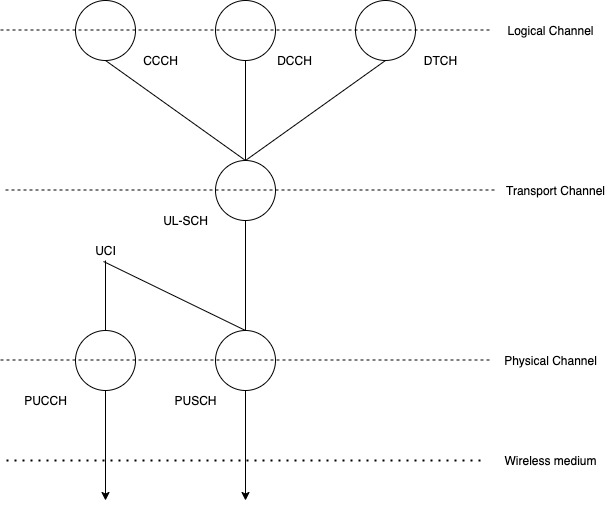
\includegraphics[
      width=8cm,
     height=10cm,
    keepaspectratio,]{uplink_scheme.jpg}
    \caption{LTE channel propagation}
    \label{fig:lte_chan_prop}
\end{figure}



To understand the process of information transfer between the eNB and the UEs, we must take not of the flow of the channels. When constructing an uplink feedback message, the data begins at the MAC layer, and is sent along the logical channel within the LTE protocol structure. Next the data is then multiplexed to the transport channel which offers information for the MAC and higher layers, via the UL-SCH. Finally the data reaches the physical channel. This outlook is important to understand where the origins of the feedback information are coming from. In LTE the physical layer itself does not decided on the feedback information, it merely is responsible for encoding and decoding. The MAC layer on the UE is where the multiplexing of data and feedback indicators the UE would transmit on the uplink about channel quality, these in the LTE framework are known are Channel Quality indicators (CQI, which will be explained in details in later sections). Other mechanisms such as data delivery verification through HARQ ACK/NACK are used to ensure the data sent was indeed received correctly. These two methods amongst others are processed in the MAC layer. \cite{3gpp25319}[Section 7]. The scope of this thesis focuses more on the physical aspects of LTE, thus outlining the main channel of importance below;
\begin{itemize}
    \item PUCCH - used for control data, this data is transmitted in the form of Up-link control information. This usually contains information related to Scheduling request, HARQ ACK/NACK and CQI. 
    \item PUSCH - this is the main user data channel, in certain conditions it also carriers the UCI and feedback metrics ACK/NACK and CQI.
\end{itemize}
\textbf{CQI} - Channel quality indicators, are as the name would suggest indicators which represent the quality of the channel at a given point in time, these are used to understand which kind of modulation the eNB should use. \newline
\textbf{ACK/NACK} - Acknowledgement and Not Acknowledgement , these pieces of information are transmitted back to the eNB to verify that the data received was not corrupted and its integrity was intact, these features will be explained in greater details in the next section.

\subsubsection{Channel State indicators}
As discussed previously, metrics or indicators about the channel are utilised in the LTE framework. The indicators are used to adjust the configurations of the transmission of data to best serve the conditions that are currently being experienced at that moment in time. 

At a high level we can group these feedback items as channel state information (CSI) , which can be broken down into; CQI - channel quality indicator, this metric gives insight into the quality of the channel at any given time. The quality of the channel can be influenced by many factors, i.e the environment, other users etc. The value of CQI can be between 1 and 15, or if the CQI index if 0 then the index of 1 does not satisfy the condition that the transport block error probability has not exceeded 0.1 \cite{ETSITS136213}[Section 7.2.3]. The CQI is then used to decide which modulation scheme to use and the relevant transport block size, depending on the quality of the transmission \cite{ETSITS136213}[Section 7.2]. 

Dependant on the configuration of the UE the aforementioned CQI feedback is realised through different architectural approaches. Both, time and frequency resources and configurations are chosen by the eNB in the serving cell region, these mechanisms can be either periodic or aperiodic \cite{ETSITS136213}[Section 7.2]. In the event of the both a periodic and aperiodic report being transmitted in the same sub frame, the aperiodic report takes priority and thus, would be only transmitted.  Depending on the scheduling mode of the UE and whether the CQI to be transmitted is either periodic or aperiodic would dictate which channel is to be used, we can see the possibilities for these in \cref{tab:cqi_aperiod_sel}
\begin{table}[H]
        \centering
     \begin{tabular}{||c c c||} 
     \hline
     Scheduling mode & Periodic CQI & Aperiodic CQI  \\ [0.1ex] 
     \hline\hline
     Frequency non-selective & PUCCH &  \\ 
     \hline
     Frequency selective  & PUCCH & PUSCH\\
     \hline
    \end{tabular}
    \caption{Periodic vs Aperiodic transmission and their respective channel.}
    \label{tab:cqi_aperiod_sel}
\end{table}
The aperiodic reporting of CQI is done on the PUSCH. On the other hand, periodic reporting regardless of the selective or non selective is done on the PUCCH. The exact type of the CQI is configured on the eNB through the RRC signalling. CQI reporting has a few distinct types \cite{umts_sesia}[Section 10.2.1.1]. 
\begin{itemize}
    \item Wideband feedback - UE reports a CQI value for the whole system bandwidth available.
    \item eNB configured Sub-band Feedback - UE transmits the entire Wideband CQI report, additionally a CQI value for each sub-band is also transmitted.. Sub-band CQI reports are encoded deferentially with respect to the wideband.
    \item UE selected sub-band feedback - The UE selects a set of preferred sub-bands of a predefined size within the entire bandwidth.  The UE reports one wideband CQI with one CQI report reflecting the average quality of the predefined size. The UE will also report the position of said sub-bands.
    
\end{itemize}

If the respective CQI field is not reserved for other purposes then the appropriate field bit can be toggled. The combinations of the triggering mechanism for this report can be viewed below \cite{ETSITS136213}[Section 7.2.1]: 

\begin{table}[H]
    \centering
     \begin{tabular}{||c c||} 
     \hline
      CSI request field & Description \\ [0.1ex] 
     \hline\hline
     '00' & No aperiodic trigger  \\ 
     \hline
     '01'  & Aperiodic report for serving cell\\
     \hline
     '10' & Aperiodic for 1st set of serving cells\\ 
     \hline
     '11'  & Aperiodic for 2nd set of serving cells\\
     \hline
    \end{tabular}
    \caption{Periodic vs Aperiodic transmission and their respective channel.}
    \label{tab:cqi_aperiod}
\end{table}
These respective trigger values are decoded by the UE on the PDCCH with an uplink DCI format in the UE specific search space \cite{ETSITS136213}[Section 7.2.1, Table 7.2].
It is worth noting that there exists a minimal reporting interval for any aperiodic transmission, which is 1 sub frame. Furthermore, when aperiodic feedback occurs with no associated transport block of user data, the UE shall utilise the PUCCH instead of the PUSCH.

As discussed earlier, periodic reporting of the CQI also occurs in LTE. UEs are semi-statically configured by the higher layers for periodic reporting of such metrics, which are present on the PUCCH apposed to the PUSCH \cite[Section 7.2.2]{ETSITS136213}. Like most features in the LTE framework, there exists an abundance of possible configurations. Like Aperiodic reporting, periodic reporting supports both wideband and ue-selected sub-band, however eNB-selected is not supported. Similarly, the type of periodic reporting is configured by the eNB higher signalling layers, RRC \cite{umts_sesia}[Section 10.2.1.2]. Periodic wideband feedback is similar to that of the aperiodic which is sent along the PUSCH, however the ue-selected sub-band is different. In UE-selected sub-band, the total number of sub-bands $N$ is divided into $J$ fractions called bandwidth parts. The value of $J$ is dependant on the system bandwidth, in this case, one CQI value is computer and reported for a single sub-band from each bandwidth part, along with its respective sub-band index.

PMI - Precoding matrix indicator is used to determine how the individual data streams (layers in LTE) are mapped to the antennas on the UE. Carefully selecting this matrix yields the maximum number of data bits that the UE can receive on across all layers. If the UE knows what the allowed precoding matrix are, then the UE can send a PMI report to suggest to the eNB the most suitable matrix to use \cite{csi_defs}.

RI - Rank indicator,  this is the number of layers and number of different data streams transmitted in the downlink. The aim of an optimised RI is to maximise the channel capacity across the entire available bandwidth by taking advantage of the each full channel rank  \cite{csi_defs}. 

\subsubsection{ACK/NACK}

Additionally the LTE framework has another form of feedback that is also transmitted on the PUCCH. The Hybrid Automatic Repeat Request (HARQ) is also utilised. The HARQ consists of two parts, firstly the ARQ in LTE is a mechanism that as the name suggests repeats the request if an acknowledgement (ACK) is not received by the sender after a predefined timeout period.  After this timeout period the receiver discards the bad packets and the sender will re-transmit. The next step is the Forward Error Correction (FEC), this process takes the malformed data packets and stores them in a buffer until the next transmission, the idea is that 2 or more packets received with insufficient information to decode them alone can be combined together in such a way they can produce a signal that can be decoded \cite{3gpp36321}[5.3.2 HARQ operation].

The list below outlines the process of encoding an ACK or NACK into the available resources, this is the process based on the specifications from 3GPP.
\begin{enumerate}\label{proc_pucch_configs}
    \item The UE would verify the configuration of the PUCCH \cite[Section 5.4]{36211}
    \item Procedure for determining PUCCH assignment 10.1 36.213 The 3GPP Specification outlines the explicit rules and combinations that the PUCCH can take. This section outlines the combinations of non/simultaneous and single/multiple cell transmission over PUCCH and PUSCH. This section also outlines the information which is to be transmitted in based on the choice of format \cite[Section 10.1]{36211}. 
    \item How the PUCCH bits should be encoded according to Table 5.4.1-1 in Section 5.4.1 of 36.211, this table outlines the modulation scheme to be adopted and the number of bits per sub frame according to the chosen format \cite[Table 5.4.1-1]{36211}.
    \item Finally, how to map PUCCH symbols to physical resources\cite[Section 5.4.3]{36211}.  
\end{enumerate} 

The HARQ mechanism in LTE is encoded into the UCI and carried usually on the PUCCH, however dependant on some conditions can also be carried on the PUSCH. The UCI format dictates the type of feedback metric to be transmitted. The chosen format allows different metrics to be multiplexed into the same message, these combinations can be viewed in \cref{tab:pucch_formats}, \cite[Section 17.3.1.2]{umts_sesia}. 

\begin{table}[h]
\centering
\begin{tabular}{||c| c||} 
\hline
PUCCH Format & Uplink Control Information (UCI) \\ [0.1ex] 
\hline\hline
Format 1 & Scheduling request (SR) (unmodulated waveform)\\ 
\hline
Format 1a & 1-bit HARQ ACK/NACK with/without SR\\
\hline
Format 1b & 2-bit HARQ ACK/NACK with/without SR\\
\hline
Format 2 &  CQI (20 coded bits)\\
\hline
Format 2 & CQI and 1 or 2-bit HARQ ACK/NACK ex CP\\
\hline
Format 2a & CQI and 1-bit HARQ ACK/NACK (20 + 1 coded bits)\\
\hline
Format 2b & CQI and 2-bit HARQ ACK/NACK (20 + 2 coded bits)\\
\hline
\end{tabular}
\caption{PUCCH formats and their properties}
\label{tab:pucch_formats}
\end{table}


%% sufficient to use the coding scheeme not further explaination. the drawbacks being the coherent - use pilots , and a lot of redunant resources being used , 12 bits of information being sent. 
The HARQ ACK/NACK procedure occurs when a the UE receives some user data on the PDSCH. The UE will then perform its integrity check on the received data and depending on the current setting will trigger a ACK/NACK response to the received payload. Upon receiving a payload from the eNB, the UE can send its ACK/NACK response on either the PUSCH or PUCCH, if there is no user traffic in the uplink then the UE will transmit its response on the PUCCH, however, if there is user traffic (this is visible when there is a valid uplink grant from the UE), the response is encoded into the PUSCH \cite[Section 11.4]{lte_advaned_mobile}. The procedures flow can be viewed in \cref{fig:ack_nack}. 

\begin{figure}[h]
    \centering
    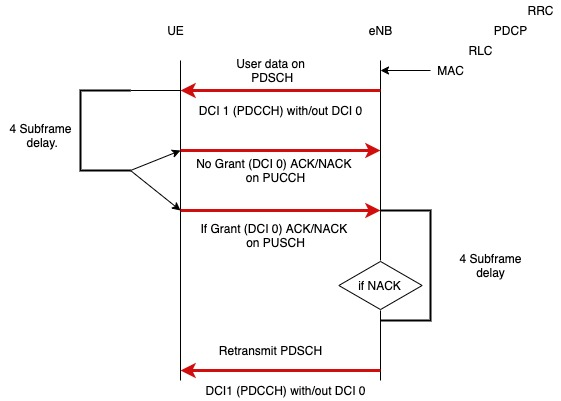
\includegraphics[
      width=8cm,
     height=10cm,
    keepaspectratio,]{ack_proc.jpg}
    \caption{LTE procedure for ACK/NACK response.}
    \label{fig:ack_nack}
\end{figure}

When the PUCCH is being utilised to transmit the feedback control data, a region of 2 resource blocks is assigned for the UE. The two resource blocks are mirrored and placed at either sides of the bandwidth to provide some integrity and spread diversity in the signal \cite[Section 11.4.1]{lte_advaned_mobile}. However, each UE having 2 resource blocks during on sub frame is much to large and not very good utilisation of resources, instead these resource blocks are shared amongst multiple UEs in a serving cell.  We can see from \cref{fig:pucchformats} that each slot (half of a sub frame), has the relevant uplink information doubly encoded at either end. If we consider the feedback for a given UE/set of UEs is transmitted we would see for example that same information is present in both cases of the $m=2$ in the \cref{fig:pucchformats}. Multiple UEs share the same regions of a sub frame mentioned before, 


\begin{figure}[h]
    \centering
    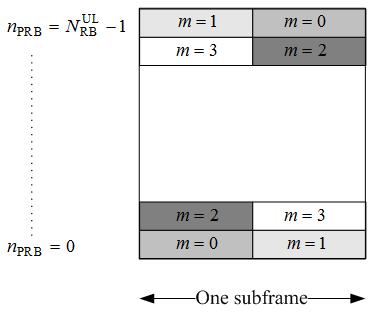
\includegraphics[
      width=6cm,
     height=8cm,
    keepaspectratio,]{pucch_formats_rbs.png}
    \caption{Resource Assignment PUCCH Format 1/2}
    \label{fig:pucchformats}
\end{figure}


As we see in \cref{tab:pucch_formats} is possible to multiplex both the CQI and HARQ ACK/NACK data from a UE to the eNB on the PUCCH, providing the higher layers have not disabled this feature, when this is disabled the UE may only transmit the HARQ. However, in sub frames where the eNB scheduler has allowed for simultaneous transmission of both metrics a multiplex of both aspects needs to be achieved. In this case there are two situations of note, for normal CP and extended CP \cite{umts_sesia}[Section 17.3.3]. 

Looking first at the multiplexing of CQI and HARQ with normal cyclic prefix (DCI format 2a/2b). To transmit a 1 or 2 bit HARQ ACK/NACK together with the CQI, the ACK/NACK bits are not scrambled, but only modulated with either BPSK/QPSK, resulting in a single modulation symbol $d_{HARQ}$.  This single modulation symbol $d_{HARQ}$ is then used to modulated the second Reference Signal (RS) symbol in each CQI slot, meaning the ACK/NACK is actually signalled through the RS itself.

% $h_1 \\
% h_2 \\
% h_K \\
% s_{1,X_1} \\
% s_{2,X_2} \\
% s_{K,X_K} \\
% z \\
% $\hat{\theta}$

% $CQI_{1} \\
% CQI_{2} \\
% CQI_{K} \\
% s_{1,CQI_1} \\
% s_{2,CQI_2} \\
% s_{K,CQI_K} \\
% ACK_{1} \\
% ACK_{2} \\
% ACK_{K} \\
% s_{1,ACK_1} \\
% s_{2,ACK_2} \\
% s_{K,ACK_K} \\
% $

%% should i add in here more information about the super specifics about subframe allocation etc???

\section{Type Based Multiple Access in LTE}\label{tbma_sec}
% this could be more context of LTE apposed to generic, 
% move the generic stuff , move into the sota. 

%  now add in the process of moving to lte. 
%  describih map in here how tbma in genreal goes to lte wrt subcarriers etc 
%  figure 6 should be an equation for s = N * R
%   remove this extra x...x1 stuff and then talk about the actual encoding , the orthogonality is achieved through using just single sc. rename section encoding scheem, how they encode the pucch or so. etc. given the available subcarriers available  - this is the story around the sota, applied to the actual LTE framework..only working for single users, ic approach has the potential for eaiser life in large numbers. 
In this section, we will go into greater detail about the system models presented in \cref{eq:system_model}, \cref{eq:simplified_system_model} and \cref{eq:system_model_retrans} which will give context in the LTE framework. We will address a couple of use cases for \ac{TBMA}, looking at both CQI and ACK/NACK feedback.
Lastly, how the parameter estimation of the TBMA in LTE is presented for both identical and fading channels. Finally, potential LTE transmission schemes are presented and discussed with applications within the LTE framework. 


If we compare back to the original \cref{fig:tbma_general}, but with the above LTE specific adaptations, we can see how this would now fit in with the new design, seen in \cref{fig:tbma_cqi}.

\begin{figure}[H]
    \centering
    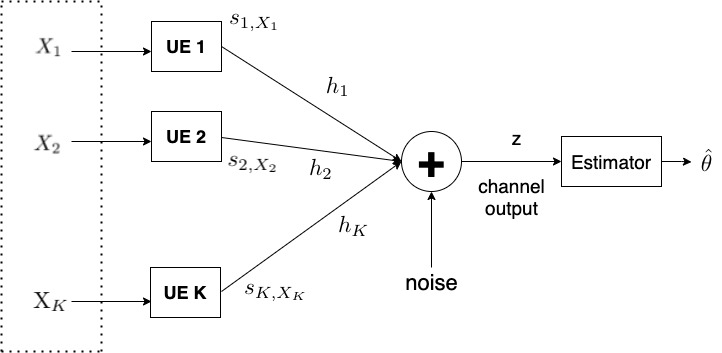
\includegraphics[
      width=10cm,
     height=10cm,
    keepaspectratio,]{sys_model.jpg}
    \caption{CQI Estimation over Multi Access Channel}
    \label{fig:tbma_cqi}
\end{figure}

We can see now how this generic \ac{TBMA} model can be built up to incorporate a variety of different real world cases. Under this new adaptation for a specific use case we would arrive to a LTE CQI specific system model for realising \ac{TBMA}. Where in \cref{eq:system_model_cqi}, the relevant terms are substituted out to allow for the source and channel coding to suit that of \ac{CQI}. 

\begin{align}
    \boldsymbol{y} = \sum_{k \in \mathcal{K}} h_k^l \boldsymbol{s}_{CQI_k^l} + \boldsymbol{w^l}, \label{eq:system_model_cqi}
\end{align}


More over, we can apply the same setup to another LTE specific use case, when each user in the group would transmit a ACK or NACK response, as described in \cref{lte_feedback_current}


\begin{figure}[H]
    \centering
    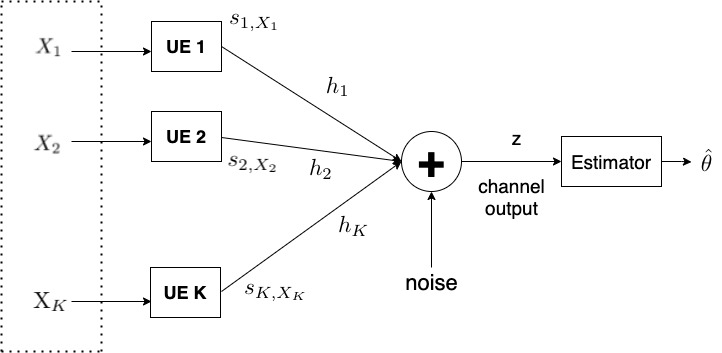
\includegraphics[
      width=10cm,
     height=10cm,
    keepaspectratio,]{sys_model.jpg}
    \caption{CQI Estimation over Multi Access Channel}
    \label{fig:tbma_cqi}
\end{figure}


\begin{align}
    \boldsymbol{y} = \sum_{k \in \mathcal{K}} h_k^l \boldsymbol{s}_{ACK_k^l} + \boldsymbol{w^l}, \label{eq:system_model_acks}
\end{align}



After observing a received signal, the fusion centre will apply matched filters to the orthonormal basis $\left\{ \boldsymbol{s}_r\right\}_{r \in [R]}$ which gives
%
\begin{align}
    \boldsymbol{z}^l &\triangleq \left[\langle \boldsymbol{y}^l, \boldsymbol{s}_1\rangle, \ldots, \langle \boldsymbol{y}^l, \boldsymbol{s}_R\rangle  \right]^T, \label{eq:mf_output}
\end{align}
% look after notations consistency - donty need the matched filter, as we have this mat
where $\langle \boldsymbol{y}^l, \boldsymbol{s}_r\rangle$ denote the inner product of the received signal and $\boldsymbol{s}_R$ at the $l$-th transmission. Where the matched filter is the scalar product of $y$ with the orthonormal signature, because the signature is orthonormal, all the other information in the signal is removed and thus is matched to the desired signature we can see this effect in \cref{fig:sig_mat}. 

There exist some constraints and assumptions for the system model. As discussed in \cref{sota}, it is assumed that the energy constraint $||s_{i}^2|| \leq 1$, where the signal of each transmission does not exceed more than 1 energy unit, this means that each user should not transmit their signal with any extra power. This will play an important role later on when we discuss the re-transmission of the signal. For example, if there are multiple re-transmissions for a given \ac{UE}, they should have the power of the entire transmission normalised.  It is also assumed that all noise and channel response (when applicable) is modelled as white complex Gaussian.   

\subsection{Data Model}\label{data_models}

Here we will present and discuss the two data models for both the ACK/NACK and CQI use case, presenting their decision matrix and discussing the applications to the LTE framework. Next, we move to a more granular approach for estimating a range of common events. Finally we take another step and look at how we could transmit and understand a PMF of real world values. 
% exchange xk by cqi_k , the index comes from the sig
%  state the size of the matrix and give dimension based on the size of subcarriers available. 
% the have definition to the matrix 
% corresponds to identity matrix and the rows are signatures and the meaning th position of the respective value in which we want to transmit.  choose signature out of big S to get the little s.  i need to loop back to the original model and then add in the specific LTE use case. 
%% CQI INDIVIDUAL
At each node one out of $R$ events occur, each event~${X_k \in \{1, \ldots, R\}}$ is draw with probability $X_k \sim$ Poisson ($\lambda$). Where the events can be correlated among all nodes or completely independent. This local event~${X_k \in \{1, \ldots, 2\}}$ is measured by each node, as there are only two possible outcomes, either ACK or NACK. Thus, the measurement vector for the ACK/NACK case is $\boldsymbol{x} \in \{0,1\}^{R}$ of each sensor node in~\ref{eq:system_model_acks} is obtained by;
% \caption{$n \times 2$ ACK/NACK Signature matrix.}

\begin{align}[H]
\centering
    $ S^{ACK} = 
    \begin{pmatrix}
    +1 & 0\\
    0 & +1 \\
    \end{pmatrix}$
% \label{fig:sig_mat_acks}
\end{align}

Here, the objective at the fusion centre is to obtain the PMF of all measured events by observing~\ref{eq:system_model}. In this case, each available subcarrier $s_{CQI}$ for a given user $k$ observes event $x$, where the encoded subcarrier of the event corresponds to a variety of actual values in the real world. This approach allows for different events to be observed and then transmitted. N


\begin{figure}[H]
\centering
    $ S^{CQI} = 
    \begin{pmatrix}
+1 & 0 & \hdots & 0 & 0\\
0 & +1 & \hdots & 0 & 0 \\
\vdots & \vdots & \ddots & \vdots & \vdots \\
0 & 0 & \hdots & +1 & 0 \\
0 & 0 & \hdots & 0 & +1 \\
\end{pmatrix}$
\caption{$n \times 16$ \ac{CQI} Signature matrix.}
\label{fig:sig_mat_cqi}
\end{figure}

The same principal can be applied also to the CQI in LTE,  where the local event~${X_k \in \{1, \ldots, 16\}}$, where 16 is the total number of possible values a CQI response can take. We can see this effect in \cref{fig:sig_mat_cqi}

\subsection{Parameter Estimation}\label{param_estimation}
%% here i talk about how to estimate the parameter or pmf of the transmitted signal, again i split this into both h=1 and random. 

As presented in the previous section, we are interested in three different data-model use cases. The idea of a TBMA  approach is to best design the channel so that the error of the estimated parameter can be minimised, such that it tends toward 0.  In some cases, we may want to determine an estimate of the actual parameter, $\theta$, in other cases we are interested in the underlying PMF, $p_{\theta}$ of the data transmitted. Respectively they are formally defined as:
% i can resuse the equations , but with the LTE specific terms to illustrate the mvoe to LTE, 
% \begin{align}
% \hat{\theta}^* = \min_{\hat{\theta}} D(\hat{\theta}\|{\theta}),      
% \end{align}
% check the poiss distr, that theta would be lambda. read about this some more. - exchange to CQI that they are random, and follow a certain distr. and we define this metrix. 
\begin{align}
{Q}^* = \min_{\hat{Q}} D(\hat{p}\|p_{\theta}),  
\end{align}

Where the min $ \min_{\hat{\theta}} D$ and $ \min_{\hat{Q}} D$ are measured using the Mean squared error, which is defined as:
% lips has the figure on the first page!! describing the appplication of cqi feedback. it has the use case of cqi describeed there already. 
\begin{figure}[H]
    \centering
\begin{equation}
  MSE = \frac{\sum\limits_{S=1}^{S}|\theta -\hat{\theta}|^2 }{S} \
\end{equation}
    \caption{Mean Square Error between Ground truth and outcome.}
    \label{fig:MSE}
\end{figure}

Where, $\hat{\theta}$ and $\hat{p}^*$ are the parameter and PMF of the received signal respectively which exist in the defined probability space $[R]$.  We assume that there is no prior knowledge of the parameter $\theta$ or $p_{\theta}$, since the idea of the approach is to derive an estimate of the distribution of the data.


\subsubsection{Identical Channel}\label{det_chan}
%  this is basically what was done in the sota, the same applies here. discuss this refering back to the sota, but maybe giving in terms of the LTE. differernt propogation channels fading. but then we can directly infere the measure from the signal 
It is assumed that the data is i.i.d between sensors but constant during different observation periods. For the specific case of identical channels ${(h^i_k = 1, \forall k)}$, the output of the bank of matched filters in \cref{eq:mf_output} contains a noisy version of the histogram, scaled by the number of users, which is presented in \cref{simple_estimation_indentical}. However we have the additional term in the LTE specific use-case, $l$, which is the number of re-transmission, thus we have the LTE specific estimator for an identical channel of:
%
\begin{align}
    \boldsymbol{z}^l &= K \tilde{\boldsymbol{p}}^l + \boldsymbol{w}^l, 
\end{align}
%
where $\tilde{\boldsymbol{p}}^l = \frac{1}{K}[N_1^l, \ldots, N_R^l]$ is the \emph{empirical measure} or \emph{type} with
\begin{align}
    N_j^l = \sum_{k \in \mathcal{K}}(X^i_k = j)
\end{align}
and $\boldsymbol{w}^l \sim \mathcal{CN}(0, {\sigma^2 \boldsymbol{I}_R})$, which is the complex Gaussian noise.
%
Therefore in the case of this deterministic channel, the estimate can directly obtain the histogram from the $l$-th measurement as:
%
\begin{align}
    \hat{p}^l &\approx \frac{\boldsymbol{z}^l}{K}. \label{eq:empf_h_const}
\end{align}

As discussed in \cref{sota}, the same assumptions apply when the number of users, $k$ and re-transmissions $l$ tend toward and away from infinity.
Although the deterministic channel is not a well rounded picture of the real world, it does however give us some insight to underlying aspects of the systems as described in the previous two a paragraphs. This information can help build up a better picture of TBMA moving forward looking into a more realistic situation in the wild.

\subsubsection{Fading Channel}\label{rand_chan}
% add in info on fading channels here
In the real world, it is more often than not less likely that a transmitted and receiver are in a direct line of sight (direct line of sight is a transmission path that is unobstructed or reflected by obstacles in the environment). An example of line of sight can be seen in \cref{fig:line_of_sight}

\begin{figure}[H]
    \centering
    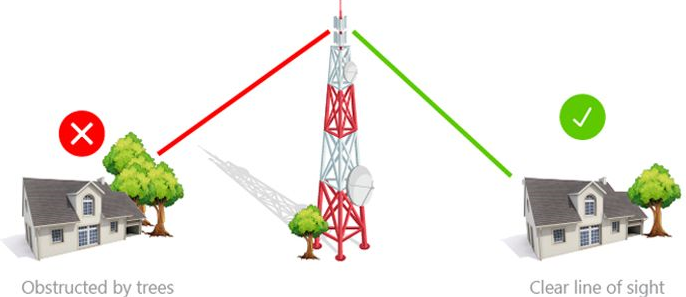
\includegraphics[
      width=6cm,
     height=7 cm,
    keepaspectratio,]{line_of_sight.png}
    \caption{Line of Sight obstruction from obstacles \cite{los_pic}. }
    \label{fig:line_of_sight}
\end{figure}

What tends to happen is that in busy environments there are obstacles such as buildings and walls that will obstruct the path of the disseminating wireless waves. The situation leads to multi path waves arriving at the receiver at different time intervals and power due to the physical affect the aforementioned obstacles have on the physicality of the waves.[ref]

This means that slightly varying waveform of the original signal are received, these can be out of phase and can be viewed from an $x$ and $y$ component, having both real and imaginary values, which can be summed to give a complete imaginary component. This effect can be viewed in Figure \ref{fig:rayleigh_fade_comps}, where the dotted lines are the different aspects of the signal received and the final complex component in bold. 

\begin{figure}[H]
    \centering
    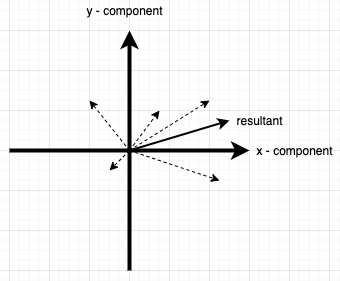
\includegraphics[
      width=6cm,
     height=7 cm,
    keepaspectratio,]{rayleigh_graph.jpg}
    \caption{Rayleigh fading components of signal. }
    \label{fig:rayleigh_fade_comps}
\end{figure}


The amount of fade for each path which is received at the user is considered to be i.i.d and based on the central limit theorem, when adding up multiple random variables for each of the $x$ and $y$ components we attain a Gaussian PDF for each of the axis. If we then consider that each of these Gaussian are independent, the overall PDF can be obtained by multiplying both PDFs together. 

With channel coefficients drawn \ac{i.i.d}. between sensors and observation intervals $h^l_k \sim \mathcal{CN}(0, 1)$, the output of the matched filter is a vector of random variables, where the \ac{PDF} of the $j$-th element is given by $p_{\mathbf{z}}(\boldsymbol{z}^l[j]; N_j)$, with  
%
\begin{align}
    p_{\mathbf{z}}(x; \sigma) &= \frac{x}{\sigma^2} e^{\frac{-x^2}{2\sigma^2}} ; 
    \newline 0 < x < \infty
\end{align} 
% lambda is mean of pois
% should i do the proof here for MLE of Rayleigh?
Where the likelihood function of the approach is detailed in \cref{glossary}

Hence, rearranging, the unbiased ML estimate of the $j$-th element of $\tilde{\boldsymbol{p}}$ can be obtained after observing $L$ transmissions as
%
\begin{align}
    \hat{p}[j] &= \sqrt{\frac{1}{2L} \sum_{i = 1}^{L}\boldsymbol{z}^i[j]}.\label{eq:empf_h_rand}
\end{align}

In other words, with a noisy, random complex channel, we can exploit the noise over multiple re transmissions of the exact same information to allow the estimator to reduce the effect of the stochastic noise allowing a more accurate reading to be obtained. As with the identical channel, we observe the same behaviour when we tend toward and away from infinity, as discussed in \cref{sota}.

\subsection{Application examples} \label{schemas_and_channels}
The idea of how best to form the TBMA channel to maximise the likelihood of estimation of the empirical data. Different use cases exist to best utilise the channel. This next section describe potential examples of application in the context of the LTE framework. First, a generic event based encoding is shown. Next examples are shown for, ACK/NACK encoding, \ac{CQI} of individual values and then finally a \ac{PMF} of \ac{CQI}.


\begin{figure}[H]
    \centering
    \textbf{Schema: Generic TBMA.}\par\medskip
    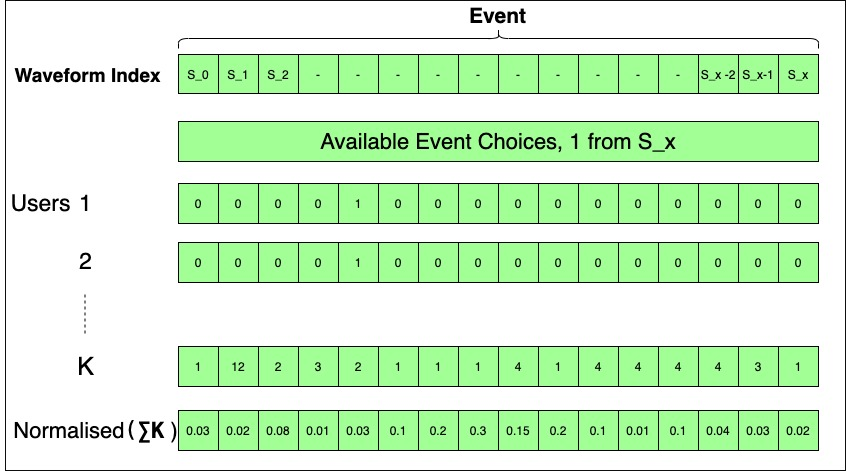
\includegraphics[
      width=10cm,
     height=12cm,
    keepaspectratio,]{system_model_tbma.jpg}
    \caption{Encoding a generic event through TBMA.}
    \label{fig:generic_events}
\end{figure}

The Schema presented in figure \ref{fig:generic_events}, shows the generic approach for taking any event and encoding it to any given available subcarrier. If we refer back to the system model presented in \cref{eq:system_model}, we can see clearly in \cref{fig:generic_events}, how the terms in the system model line up. It now becomes more apparent how the joint channel and source work in unison. We can clearly see in \cref{fig:generic_events}, that multiple users can choose a signature, depending on the observation that respective user has made, in simplistic terms we can see the summed outcome of all users choices. Referring to \cref{fig:generic_events}, we  see at the $K$-th element we have multiple users who have chosen for example, the same observation. If we refer back to \cref{fig:pmf_subcarriers}, we can see how this $K$-th element without a channel or noise would translate to a \ac{PMF}. Thus, through all users adhering to the same scheme, we arrive at the bottom of the diagram at the fusion centre where we receive the normalised combination of all the transmitted waveforms from all the users in a group. 

Now that this has been clearly illustrated in general TBMA terms, we move now onto applying this a LTE specific example. First if we refer back to \cref{eq:simplified_system_model}, where the channel is identical and we do not consider and re-transmission. We can see this paradigm shift from generic waveforms to LTE subcarriers in \cref{fig:generic_lte_events}.

\begin{figure}[H]
    \centering
    \textbf{Schema: Generic LTE event.}\par\medskip
    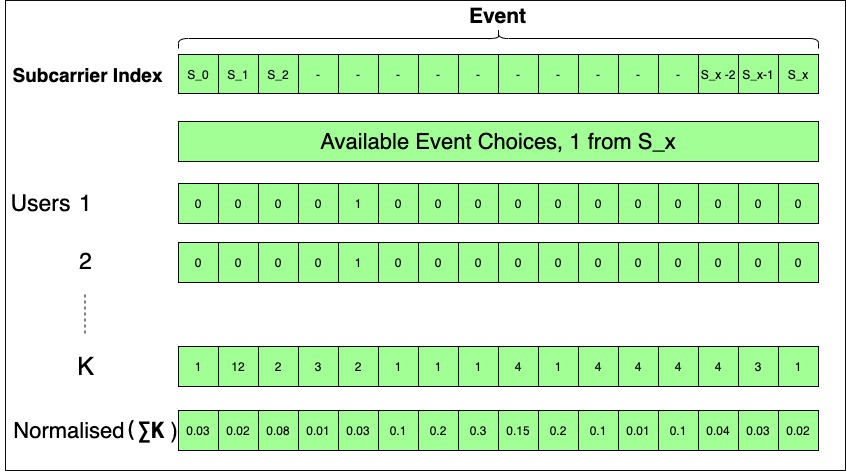
\includegraphics[
      width=10cm,
     height=12cm,
    keepaspectratio,]{lte_scheme_simple.jpg}
    \caption{Encoding a generic LTE event through TBMA.}
    \label{fig:generic_lte_events}
\end{figure}

The Figure \ref{fig:generic_events} has the same notation as Figure \ref{eq:system_model} to help visually understand how the equations fit together. The same constraints for the equations apply. Any user in the network can take any available subcarrier, $S$, and encode a single bit which correspond to that of an event in the real world. These events could correspond to any real world values, providing all the users in the network assume the same encoding style. During for example,  a multicast it would be beneficial for the \ac{eNB} to understand if the majority of users in a multicast group have received the message correctly. 

To do so, a simple ACK or NACK response could be elicited by each user for the eNB to understand if the message was received by all \ac{UE} and whether that information was received correctly, or not. However given current feedback approach described in \cref{sota}, using the \ac{PUCCH} or \ac{PUSCH} for each user in the group, this would entail as discussed in \cref{prob_context} a single resource for each user in the group, which as we have shown is not ideal.
 
Consider, a group of $1000$ \ac{UE}, $k$, where each UE transmit their feedback current uplink feedback methods discussed in \cref{lte_feedback_current}. Under this approach each UE would take time $t$ to transmit each ACK/NACK response on a dedicated channel. This may not be such a issue for small to medium sized groups. However, for larger cell regions, this would be a time consuming, resource intensive task and is it not efficient. Contrarily, using the likes of TBMA could mitigate these resource issues. The current approach in LTE has a one to one mapping of resource to UEs, using TBMA we could have a many to one mapping - i.e. $1000$ users would take collectively time $t$, apposed to needing time $t$ for each user. In LTE ACK/NACK is an automatic response, mixing this with multicast transmission becoming more common we can clearly see time $t$ vs number of UEs $t$ is a huge advantage as the number of users in a group grows. 

\begin{figure}[H]
    \centering
    \textbf{Schema: Encoded ACK/NACK}\par\medskip
    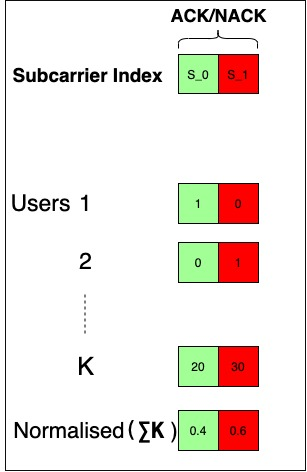
\includegraphics[
      width=6cm,
     height=6cm,
    keepaspectratio,]{ack_nack_lte.jpg}
    \caption{ACK/NACK encoding on 2 subcarriers}
    \label{fig:acknack}
\end{figure}

\cref{fig:acknack}, shows a simple coding scheme where two available subcarriers could encode exclusively either an ACK or NACK depending on what the specific UE has observed at that point in time.

% Figure \ref{fig:ack_schema}, shows how the above process could work. By spreading each users ACK signal across the available subcarrier range. we could introduce signal diversity, by each user choosing more than one subcarrier and encoding. The idea would be to reduce the effect of noise is and concentrate noise on a specific subcarrier, rather this is spread out across all available. This would reduce the the weighting of noise when the normalisation of the signal happens, giving us a more realistic estimate. 




% \begin{figure}[H]
%     \centering
%     \textbf{Schema: Encoded Halves, Each User XOR ACK-NACK}\par\medskip
%     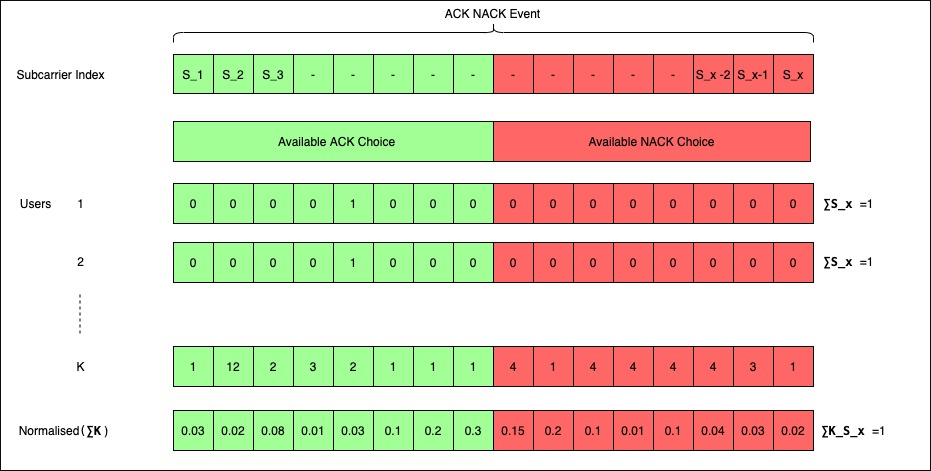
\includegraphics[
%       width=10cm,
%      height=12cm,
%     keepaspectratio,]{ack_halves.jpg}
%     \caption{Halved One shot random XOR allocation of subcarriers, from 1 user to N. }
%     \label{fig:xor_schema}
% \end{figure}

% The schema depicted in \ref{fig:ack_schema}, has some drawbacks. If we do not know the size of the multicast group then it would be hard to gauge how many users have successfully received the intended transmission, additionally without the NACK element of the feedback, it would be hard to gauge how the overall consensus about the channel is. For this reason, an additional architectural aspect could be introduced. By adding another dimension to the scheme, the NACK field and Splitting the available subcarriers into two halves could allow for a more granular understanding of the current state of the system, having a situation where comparative values are available allows for some interesting information to be extracted. 

If we take the example of autonomous vehicles in a smart city, where there are a lot of users, pedestrians, potential interference and reflection from buildings and other wireless communication. In this kind of environment, it may be understandable that some data received is corrupt and incomplete. In these safety critical situations, where inevitably there will be multiple sets of grouped users who would be receiving many messages about updates in their environment. This kind of scenario clearly needs to have ACK/NACK feedback to ensure that dropped message and successfully re-transmitted and received, otherwise incurring potential dangerous situations 

% For example, if there are an unknown number of cars $C$ in a cell region and the fusion centre receives signal, $Z$ of the TBMA channel using Figure \ref{fig:xor_schema}, then the base station could understand a ratio of the integrity of the received data for all of the users, consider;

% \begin{align}
%     Ratio_\text{ACKs} = \frac{Z_{0}\ldots Z_{\frac{S}{2}}}{Z_{\frac{S}{2}}\ldots Z_{S}}
% \end{align}
% %  put this to the end and maybe not saying exact. don't make more problems for myself. only discuss in an examples , dont leave open questions. 
% Where $S$ is the total number of subcarriers available in that channel construction, this approach would allow the base station to understand what proportion of the total number of users is receiving well formed data packets. Further information could be extracted if it is assumed that each user transmits with the same energy, $E$, then the base station knows what energy each user is transmitting with, thus the total energy received by the fusion centre;

% \begin{align}
%     Z_{K}  = K \cdot E_{k} + w
% \end{align}
% \begin{align}
%     \implies K \approx \frac{Z_{K}}{E_{K}}.
% \end{align}

% Where the number of users can be approximated based on the total energy of the received signal, this holds true because of the energy constraint discussed in \cref{sys_mod}, this is an approximation because of the additive nature of noise in the transmission. 

As discussed in \cref{sota}, a very useful piece of feedback information each UE can give the eNB is the Channel quality indicator (CQI), which was discussed in \cref{lte_feedback_current}, The CQI is, as the name suggests an indication of the quality of the channel each user is experiencing. This CQI value allows the eNB to best understand which modulation scheme to use for transmission. The CQI value ranges from 0-15 (modulation from QPSK to 64QAM), with 0 meaning the UE is out of cell range and 15 being the best case scenario. This is a very useful tool for the eNB to understand how efficiently depending on the external environmental factors to encode the information along the channel. 

The same situation applies here as the ACK/NACK scenario, the users should best use the channel to convey the collective consensus on the quality of the channel, with potentially huge amounts of users in a cell region, the feedback from multicast could be hard to handle. Using a TBMA channel with 16 subcarriers, each user could transmit an encoded bit in their respective subcarriers which corresponds to a real world value for the CQI. Case II from the data model is illustrated here, each user has a common set of different values which can be taken. 

\begin{figure}[H]
    \centering
    \textbf{Schema: CQI Individual structured encoding}\par\medskip
    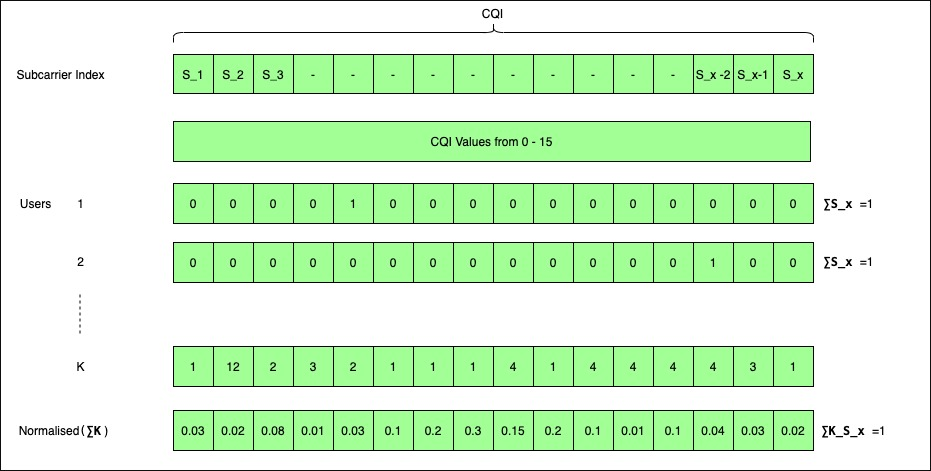
\includegraphics[
      width=12cm,
     height=14cm,
    keepaspectratio,]{CQI_individual.jpg}
    \caption{Transmitted encoding of user gathered CQI information. }
    \label{fig:cqi_ind}
\end{figure}

As seen in Figure \ref{fig:cqi_ind}, each available subcarrier corresponds to a real world CQI value. This approach allows the eNB to get a snapshot of the current quality of the channel from multiple users. The eNB would receive at its fusion centre a PMF of the group of users CQI values at that instant, this would provide an overview of how all users in a group are receiving in the channel and allow the eNB to more appropriately adjust its encoding scheme to suit the majority of users. Circling back to one of the huge benefits of TBMA, as with traditional feedback methods 

Finally, the proposed channel on Figure \ref{fig:cqi_ind} is not without fault, error in the world of measurements is something that cannot be avoided, for this reason when measuring anything it is good practice to take a set of measurement to iron out any anomalies which may have occurred. 

Therefore, a step further for the CQI which could yield more stable and realistic results for the quality of a channel over time could be each user transmitting a recorded PMF of their respective CQI over time. This approach can be viewed in Figure \ref{fig:cqi_pmf}. This approach might be more realistic than its counterpart in the previous paragraph, due to the fluctuating nature of CQI in an outdoor environment. With the eNB having a more generalist snapshot of the CQI overtime vs an instantaneous approach could avoid unnecessary modulation coding changes when they are not needed. 

\begin{figure}[H]
    \centering
    \textbf{Schema: CQI PMF encoding}\par\medskip
    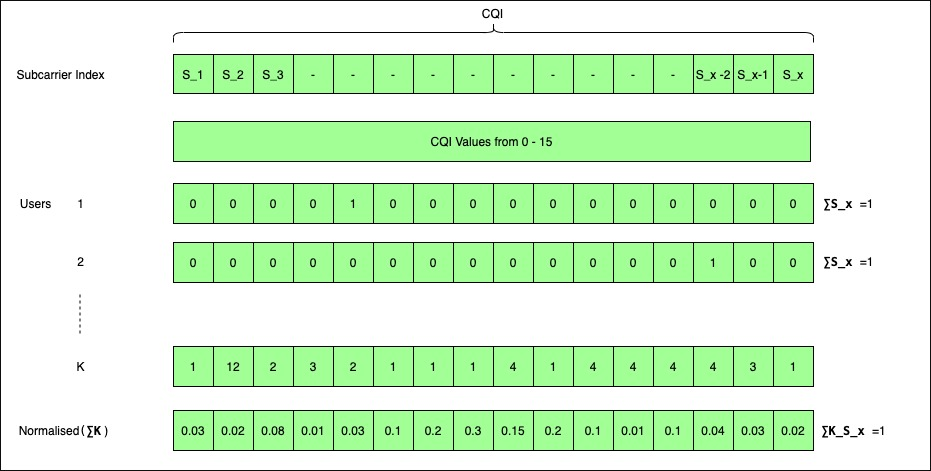
\includegraphics[
      width=12cm,
     height=14cm,
    keepaspectratio,]{CQI_individual.jpg}
    \caption{Transmitted encoding of user gathered CQI information. }
    \label{fig:cqi_pmf}
\end{figure}

It is worth noting that in the case of this approach, that the total number of energy of each transmission is constant. Therefore, each users PMF of measurements for a given $l-th$ transmission must satisfy:
\begin{align}
    E = \sum \boldsymbol{s}_{X^l_k} 
\end{align}

Such that if a user $k$, transmits a PMF of CQI values, each encoded subcarrier must only have $\frac{1}{X}$ proportion of the total energy available for each user. This is an important consideration and assumption to allow for further analysis of the received signal. 

As different scenarios are presented, some return higher levels of granularity than others. Above, some scenarios have been presented where only general information about ratios are of interest, however the scheme presented in Figure \ref{fig:cqi_pmf}, touches on how we can deduce more accurate types of information, these encoding and transmitted channels would not only allow the base station to understand which region of CQI users are in, but also as each user transmits a PMF, potentially we could also understand the variance of their channel quality.  Overall we can see that this goal orientated approach can indeed be tailored to the specific needs of each individual use case. As TBMA utilises this joint encoding and goal orientated approach, we can clearly see that given some consideration, sensible choice of scheme design, the TBMA approach could be adopted to fit a plethora of needs. Although some drawbacks exist that the channel and source need to be known before hand and this decreases somewhat the levels of flexibility.

\section{Application to the LTE framework}\label{lte_app}
\subsection{Introduction}
In this section we will introduce the different ways a multicast transmission can be achieved, giving an overview of the three possible methods of multicast in the LTE framework. Then the process of implementing TBMA approach in the Long term evolution (LTE) framework is investigated and discussed, Looking at the different protocol layers and architecture. The given use-case of using TBMA as a feedback mechanism for multicast transmission as of the time of writing this thesis is not yet present. This section will progress through the different aspects of the LTE framework to investigate how such a feature could be consolidated with the current implementation. In section \cref{lte_feedback_current}, we examined how feedback is currently implemented is investigated with respect to CSI and ACK/NACK information, this section will outline how this can be adopted to serve TBMA for a use case such as ACK/NACK, in particular how the integration of PUCCH format 1A could be achieved for TBMA.

The LTE framework which is an ongoing development project of the 3GPP (3rd Generation Partnership Project), it was first proposed as an international standard in 2004 by NTT Docomo of Japan. Since its inception in 2004, the LTE framework has been developed internationally and has become a standard framework for mobile radio communication, the LTE works as an intermediary framework that connects mobile users to the internet. The scope of this thesis, looking into TBMA as a feedback mechanism from multicast transmission does not exceed the elements of the UE and the eNB in the LTE context, these can be viewed below in the figure.

\begin{figure}
    \centering
    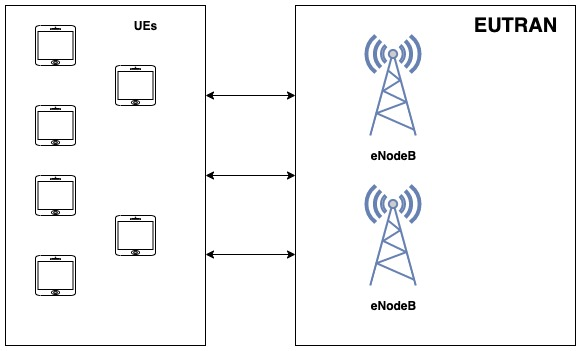
\includegraphics[
      width=6cm,
     height=7cm,
    keepaspectratio,]
    {enb_ue_arch.jpg}
    \caption{General overview of LTE Architecture.}
    \label{fig:lte_arch}
\end{figure}

This simple overview consists of a base station (evolved node b, or eNB) and then all the connected user equipment (UE), which could be an entity connected to the LTE network which is not an eNB. The LTE network is responsible for decoding, encoding and exchanging information between the users through the IP network. 

The LTE framework is broken down into different layers which are all responsible for different aspects of the life cycle of the data, within the scope of this thesis, we are concerned with Layer 1 ( the physical layer) and part of Layer 2 (primarily the MAC), these entities correspond to the layers spoken about in \cref{lte_feedback_current}. 

\begin{figure}[h]
    \centering
    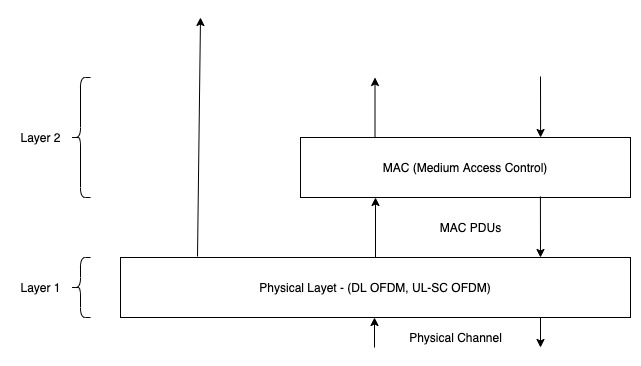
\includegraphics[
      width=6cm,
     height=7cm, 
    keepaspectratio,]
    {lte_layers_arch.jpg}
    \caption{LTE protocol layers overview.}
    \label{lte_protocol_stack}
\end{figure}

As seen in \cref{lte_protocol_stack}, the aspects of the LTE stack we are interested in are:
\begin{itemize}
    \item Physical layer (PHY) - The physical layer is responsible for all things physical, modulation, power control, link adaption and the physical encoding of the symbols. It communicates data with the MAC layer and receives control data from the RRC.[ref]
    \item Medium access control (MAC) - MAC is responsible for mapping data between logical channels and transport channels. The MAC handles all the multiplexing from logical to transport channels.[ref] The MAC layer is responsible for the 'when' the feedback mechanisms is used. 
\end{itemize}

Now the basic understanding of how the LTE framework works, with attention put on the notable aspects of the stack as discussed above, to move forward with the TBMA approach, we should understand how unicast vs multicast (SCPTM and eMBMS) works.


In unicast the base station (eNB) sends distinct messages to each \ac{UE} as depicted in \cref{fig:unicast_vs_mutlicast}. To allow this individualistic message transmission each \ac{UE} must have its own unique C-RNTI (Cell - Radio Network Temporary Identifier) as an identifier. The \ac{crnti} is used to scramble the downlink traffic (through the PDSCH) on a sub frame basis for that specific \ac{UE}. That means, that no other UEs in that cell region can decode that respective sub frame, instead any information which is not specific that UEs particular \ac{crnti} is ignored. The CRNTI is attain by each UE when it enters a cell-region \cite[Table 7.11]{3gpp36321} or in the random access procedure.  

The LTE framework is not limited to unicast transmission, two forms of multicast are also possible. Firstly we will look at MBMS, which unlike unicast utilises another primary channel called the physical multicast channel (PMCH), which is used for evolved multimedia broadcast multicast service (eMBMS). One notable difference between these two approaches is that eMBMS cannot be multiplexed with unicast, this is due to the structure of their sub frames differing. The multicast data from eMBMS is usually transmitted from many synchronised base station at the same time, this mode is called Multicast Broadcast Single Frequency Network (MBSFN)  

Unicast - As the name suggests, this is a one-to-one transmission , where each transmission is a direct channel from the sender to explicitly one receiver, this approach takes the intended users RNTI and scrambles the payload so that the data is only receivable by the intended user. This approach means that for every transmission across unicast a corresponding radio resource is also needed, this has some obvious redundancies, given the repeated usage of a radio resource, regardless of multiple users have the same corresponding information. Unicast in the LTE framework is the most frequented method of transmission. If we take each bidirectional arrow as a radio resource for general downlink data and uplink feedback data in \cref{fig:unicast_vs_mutlicast}, we could clearly see how each additional user given the current unicast feedback approach begins to use huge amounts of resources. For the multicast, if TBMA was adopted, only a single resource could be used for multicast data and feedback, severely reducing the overhead on the network for grouped data. 


\begin{figure}[h]
    \centering
    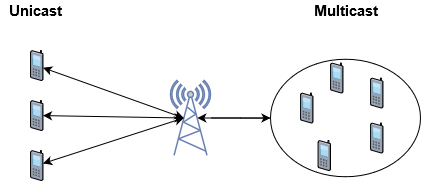
\includegraphics[
      width=9cm,
     height=10cm,
    keepaspectratio,]{uni_cast_multi_cast.png}
    \caption{Unicast vs Mutlicast with TBMA,}
    \label{fig:unicast_vs_mutlicast}
\end{figure}

% Multicast - This style of transmission, is a one to many relationship. Users are grouped together, then a data transmission is disseminated amongst all users. This style of transmission in LTE network can be achieved through a variety of ways. 
% \begin{itemize}
%     \item Unicast transmission can be done to all users in a group individually (inefficient use of radio resource as there are many duplicates of the same data based on the group size).
%     \item eMBMS - evolved multimedia broadcast service, this approach blocks a slot of the available sub frames and each user in the group has the relevant information to decode the data payload. This approach can simultaneously reach multiple users, but the scheduling of the downlink frames is very inflexible. 
%     \item Single cell point-to-multiple point (SCPTM) - this is an amalgamation of the eMBMS and unicast, this approach best utilises the radio resource, whilst reaching multiple users in one transmission.  This approach allows flexible scheduling of the resources and keeps the radio overhead to a minimum. 
% \end{itemize}

Feedback for unicast. Currently as of the 3GPP implementation, feedback for unicast transmission is still on a one-to-one topology (can be seen in \cref{fig:unicast_vs_mutlicast}), examples of feedback information the the base station would receive from this one-to-one approach, the following aspects are discussed in earlier sections;
\begin{itemize}
    \item HARQ ACK/NACK
    \item CQI
\end{itemize}

Currently whilst writing this thesis, feedback metrics for the other transmission styles mentioned earlier both rely on the same method that is used in unicast style transmission. 

\subsection{Application of TBMA to LTE}

To understand how the an implementation of TBMA could work, we need to understand data progress from human readable format to being encoded and mapped and transmitted along the channel.
To apply TBMA to feedback mechanisms in the LTE framework, the process of how LTE work encoding and decoding the signal must be understood. In modern LTE systems, OFDM (the encoding process of OFDMA discussed in the SoTA) is used to encode data in parallel to be transmitted along the channel. With the process of OFDM in LTE in mind, to realise TBMA a similar sequential encoding and decoding paradigm could be adopted. The previous section we have discussed how to implement TBMA and estimate its parameters, which is the basis of how then to apply this to the LTE framework. Looking at  \cref{fig:tbma_lte_view}, the basic flow of encoding TBMA packets can be seen. 

\begin{figure}[h]
    \centering
    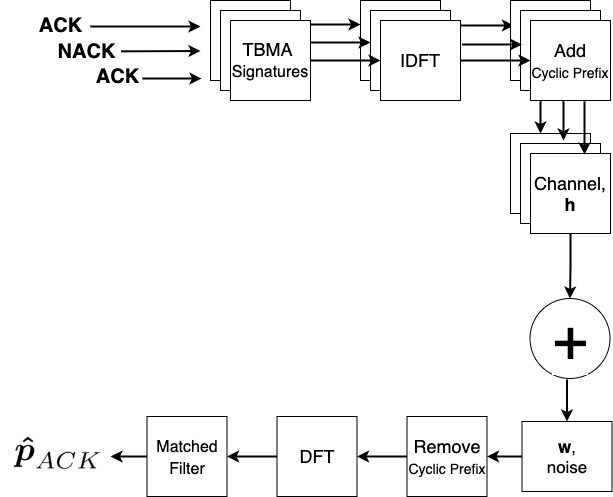
\includegraphics[
      width=6cm,
     height=7cm,
    keepaspectratio,]
    {block_diag.jpg}
    \caption{TBMA LTE overview.}
    \label{fig:tbma_lte_view}
\end{figure}

Like the current OFDM approach, both IDFT/DFT and add/remove CP are still present. However, due to the nature of this information centric multiple user simultaneous transmission approach, we can view the parameter $\theta$ or $PMF$ signatures being sent in parallel along the same channel by multiple users, unlike OFDMA there is no need to equalise or do channel estimation as we are more interested in the correlation of the values which have been sent independently from the users and thus inherently been summed over the air.
% this is achieved through the matched filter, discussed in the \cref{sys_mod}.[REF]

Next as per \cref{lte_feedback_current}, we can see how the resource elements are encoded as per the usual standard, in the scope of this thesis, a simple mechanism is to be researched to encode the ACK/NACK for multiple users for TBMA.

As the scope of this proof of concept implementation in this thesis is limited to Format 1A on the PUCCH, a graphical representation of this process has been shown in \cref{fig:pucch_encode_decode_tbma}. The process for encoding an ACK/NACK on the UE side would remain the same, the UE would encode this 1 bit piece of information into the symbols highlighted in \cref{fig:pucch_encode_decode_tbma}, this PUCCH is then put through an IFFT and sent along the wireless channel, on the eNB side the reverse is then done, FFT and decode the of the signal. However at this point is where the TBMA would be divergence from the usual approach of the feedback over unicast. At this point after the PUCCH is begun to be decoded, we would take these scalar values of the ACK/NACK which are converted from raw symbol to real values and used as correlations to tell whether the received value is indeed an ACK or NACK, these are then summed and normalised as per the original TBMA equation in \cref{sys_mod}.


\begin{figure}[H]
    \centering
    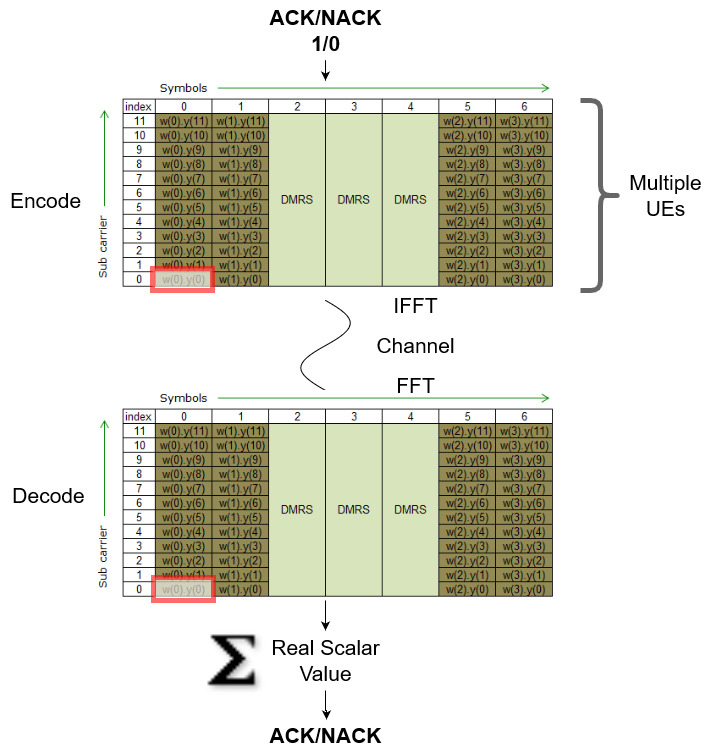
\includegraphics[
      width=11cm,
     height=17cm,
    keepaspectratio,]
    {tbma_pucch_prop.jpg}
    \caption{TBMA srsLTE process.}
    \label{fig:pucch_encode_decode_tbma}
\end{figure}


\subsection{Proof of concept}\label{srslte_poc}
This section discusses a walk through of how a Proof of concept (POC) TBMA was achieved in an LTE compliant software framework, called srsLTE mentioned throughout the thesis. Here, we will describe the tools used to perform this test in a real LTE framework and how the test is validate and evaluated. The srsLTE project is modular library and full stack SDR implementation on the LTE network. This is LTE compliant and adheres to the standards dictated in the 3GPP specifications. The srsLTE project has developed not only a full stack for Evolved Packet Core, evolved Node B and the user equipment. But, they also have exposed a modular library which can be used to piece together different aspect from within the full stack. They also offer many example code files, which can be adapted to suit the users needs \cite{srsLTE}. 

The people at srsLTE have exposed smaller unit cases for subsystems within each of the stacks. They allow quick prototyping and proof of concept coding, in particular this POC was based on their example file for $PUCCH ca TEST$, which is an example of how the PUCCH could be encoded and decoded in normal LTE operation. This example does not transmit any data over a physical wireless medium, rather it uses the same functionality as the production version of the stack until the point where the data is transmitted across the actual USRP. This means that there is no physical channel and if left as is, would equate the same scenario as described in \cref{det_chan}, however this can be adapted by programmatically adding in a random complex channel as described in \cref{rand_chan}, both approaches were tried and tested. 

This example file allows for prototyping different configurations which are validated by the srsLTE stack functions. The modular functions used allow the user to try all the combinations of the PUCCH or PUSCH configurations based on the 3GPP specification, 36.211 Section 5.4, as described in the earlier sections. The example file follows the same setup procedure which would be found in the fully functioning UE/eNB setup for encoding and decoding the PUCCH/PUSCH - we are however, only interested in the PUCCH for this scope. The relative aspects of the eNB and UE are initialised with their respective configurations. The setup of resource configurations of the tests were as follows:

\begin{itemize}
    \item Physical resource blocks = 6
    \item Transport blocks = 1
    \item Carriers = 1
\end{itemize}

After this, each UE is to encode just one ACK or NACK message at random, a comparable situation as found in \cref{schemas_and_channels}. This data is is then sent through the pipeline as would be encoded in the real world in an LTE network. The approach initially follows the same procedure for encoding the ACK/NACK bits to the PUCCH on Format 1A, however, some changes needed to be made to accommodate TBMA style feedback. The general process for encoding to the PUCCH is as follows;

\begin{enumerate}
\label{encode_pucch_proc}
    \item ACK or NACK chosen.
    \item Verify PUCCH configuration as given in Section 5.4 36.211 
    \item Procedure for determining PUCCH assignment 10.1 36.213
    \item Encode bits - dependent on Format - 1A is a straight copy of the bits. 
    \item Encode PUCCH bits according to Table 5.4.1-1 in Section 5.4.1 of 36.211
    \item Map PUCCH symbols to physical resources according to 5.4.3 in 36.211
\end{enumerate}
 
The steps to be followed are the same as shown in \cref{fig:pucch_encode_decode_tbma}. TBMA would follow the similar steps as \cref{encode_pucch_proc} with a few caveats to understand adhere to TBMA principals. With TBMA, the available subcarriers for the transmission in the case of the ACK/NACK have predefined meanings, i.e 1st available signature is for ACKs, second available for NACKs.

\begin{figure}[h]
    \centering
    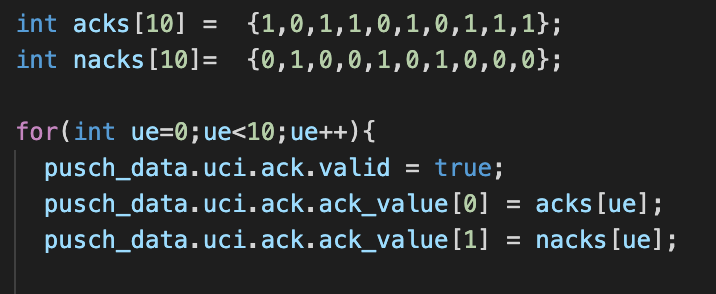
\includegraphics[
      width=10cm,
     height=7cm,
    keepaspectratio,]{acknack_creation_encode.png}
    \caption{Creation of ACK/NACK message to be encoded.}
    \label{fig:encodeACKSNACKS}
\end{figure}

\cref{fig:encodeACKSNACKS}, details how for example in this proof of concept file, 10 UEs would have their ACK/NACK subcarriers encoded. As per the previous schema ideas, the first symbol being ACK and second being NACK is depicted by $ack_value[0]$ and $ack_value[1]$ respectively, as discussed previously the encoding and transmission of these fields are mutually exclusive, meaning it would be contradictory for a UE to encode both ACK and NACK as a feedback message. The arrays in \cref{fig:encodeACKSNACKS} depict the choice of ACK and NACK for the 10 UEs in the test. 

The next step is how to physically encode these values in the the PUCCH. Configurations for format 1A are still chosen as the path through the source code. Some modifications are then made to the how these bits are encoded into the UCI. This can be viewed in \cref{fig:uci_mod_tbma}

\begin{figure}[H]
    \centering
    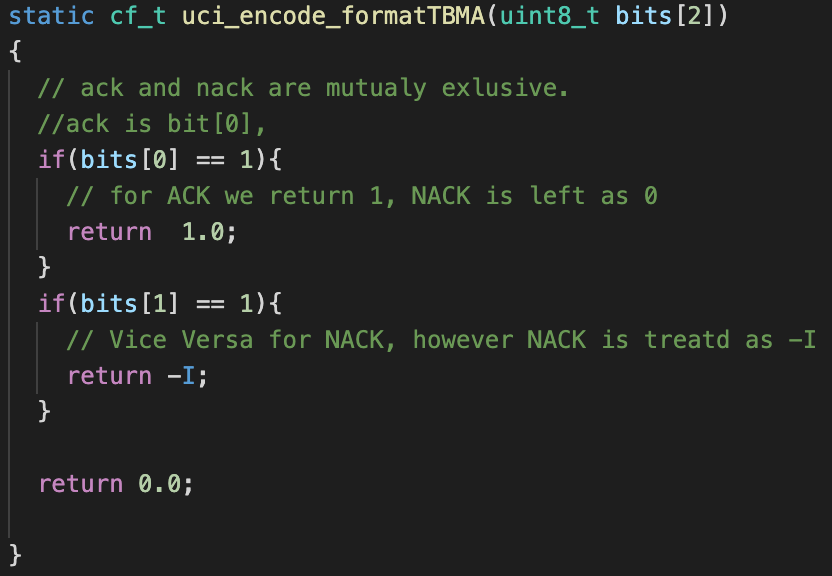
\includegraphics[
      width=7cm,
     height=5cm,
    keepaspectratio,]{UCI_encode.png}
    \caption{Creation of ACK/NACK message to be encoded.}
    \label{fig:uci_mod_tbma}
\end{figure}

Post the encoding of the UCI bits to the PUCCH, the rest of the procedure for creating the raw symbols to be transmitted is as normal. The next step in the proof of concept is deal with all the different symbols from the different users who would be transmitting the TBMA over the air. In the real world these symbols would be summed over the air by the fact they had been encoded in the same place on the actual radio link, as there is no actual radio link in this concept, the idea was adopted to sum these symbols up before they were processed on the eNB. \cref{fig:tbma_buf} can be seen that each of the symbols is just summed to there respective next users symbols, there are 1008 raw symbols due to the configurations. 

\begin{figure}[H]
    \centering
    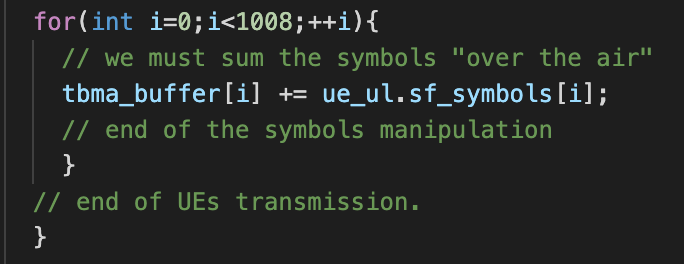
\includegraphics[
      width=7cm,
     height=5cm,
    keepaspectratio,]{tbma_buf_sum.png}
    \caption{Creation of ACK/NACK message to be encoded.}
    \label{fig:tbma_buf}
\end{figure}

At this point, we have all our symbols gathered up from multiple UE transmissions. The next step is we must process these symbols to get some useful information from them, this snipped is depicted in \cref{tbma_decode}. As we are decoding two different bit fields, which potentially could have the possibility of being 4 distinct combinations of events, i.e ack/ack, nack/ack etc, however as we know the outcome of TBMA in this case is a mutually exclusive event by  each UE, i.e each UE can only transmit either an ACK or NACK and not both, we are only interested in 2 outcomes when we match the correlation. The correlation matching is taken by finding the maximum value for the 4 possibilities that exist, then taking this as the max correlation that the value is in deed the value that was sent. These two correlation values are then taken to show what the ratio of the i.e ACKs to NACKs are.

\begin{figure}[H]
    \centering
    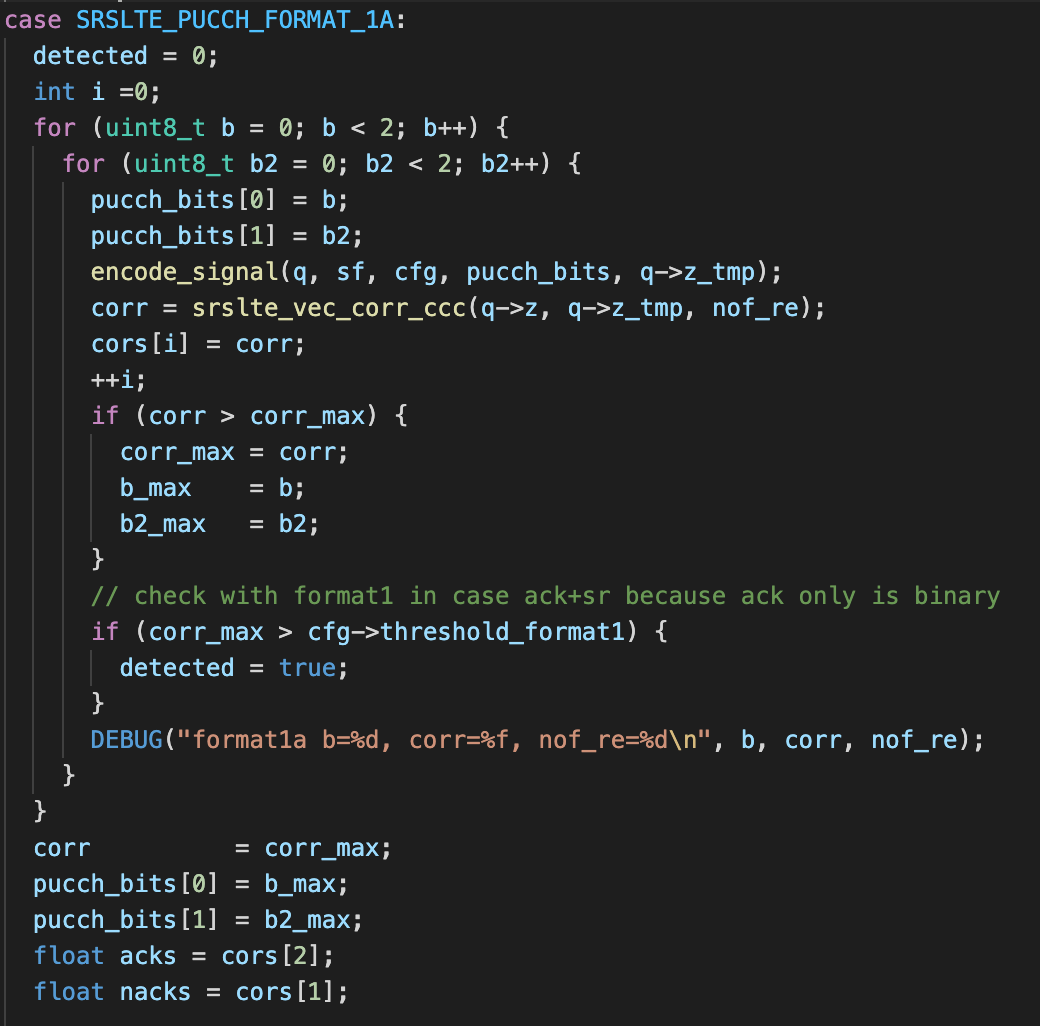
\includegraphics[
      width=9cm,
     height=7cm,
    keepaspectratio,]{decoding_tbma_acks_nacks.png}
    \caption{Decoding of ACK/NACK message transmitted over combined channel.}
    \label{fig:tbma_decode}
\end{figure}


Although there is no real radio link in this POC, it can still be made more realistic however, by adding in a simulated random complex channel as per the simulation in the previous section. The channel, h is taken from a normal distribution with mean 0 and standard deviation 1 (for both the real and imaginary parts) and applied \ac{i.i.d} along the channel of each user. Taking a step forward to a more realistic setup as per the simulations in \cref{sys_mod}, we add in the duplicate re-transmissions and the random channel, seen \cref{fig:retries_ota_complex}. 

\begin{figure}[H]
    \centering
    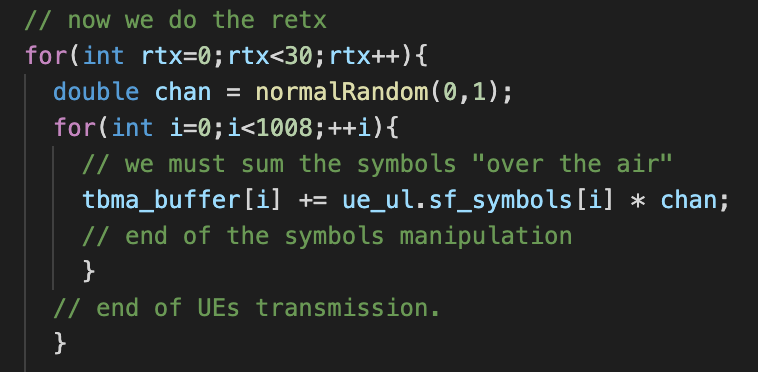
\includegraphics[
      width=9cm,
     height=7cm,
    keepaspectratio,]{retries_ota.png}
    \caption{ User Re-transmission, complex channel.}
    \label{fig:retries_ota_complex}
\end{figure}


Finally, to satisfy the power constraint on the transmission discussed also in \cref{sys_mod}. The final buffer of symbols represented by $tbma buffer$ are then divided by the number of re transmissions which were done, this is to simulate the power of the symbols being collectively worth 1 transmission vs how they would be worth 30 transmission of power. This can be viewed below;

\begin{figure}[H]
    \centering
    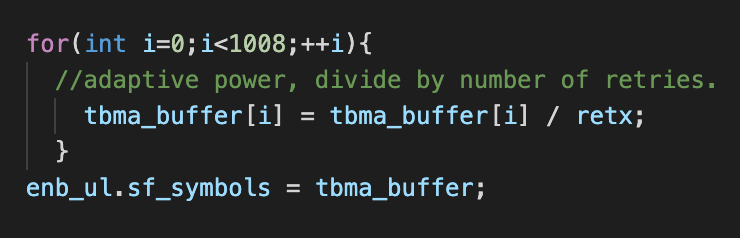
\includegraphics[
      width=7cm,
     height=5cm,
    keepaspectratio,]{adapt_power.png}
    \caption{Adaptive power of transmission.}
    \label{fig:retries_ota_complex_adapt}
\end{figure}

Overall the POC has shown that the goal-orientated approach of TBMA can be work with that of the LTE network, the implementation described above can handle encoding and decoding ACK/NACK TBMA transmission with a single signature for each ACK and NACK. It follow the same procedure which would be found in a live LTE network implemented by srsLTE, with some caveats on how the encoding is performed. Obviously some deviation was needed to achieve the decoding of the channel, however there has been nothing which based on the research done in this thesis has violated any serious LTE concerns.  

% The received symbols are then summed as per the simulation in \cref{sim_results}. As the creation of the symbols in the srsLTE stack is as per the process described earlier in the \cref{lte_feedback_current}, when inspecting the raw symbols denoted by complex floating point types with real and imaginary parts, we can sum these in the correct position as per the specification. This allows us to take all the raw symbols which would be transmitted during a multicast feedback and inspect them on a symbol basis to work out what the overall consensus of a parameter is. 


\section{Results and analysis}\label{sim_results}

This section details the results, analysis and evaluation of both the numerical simulation and also the \ac{POC} in the srsLTE SDR environment. Firstly the simulation environment section will detail the numerical analysis of TBMA, comparing the effect of different users and re-transmissions for both an identical and fading channel. Next we will move onto the \ac{POC} in the SDR environment through srsLTE, this section walk through the steps needed to realise multicast feedback through TBMA in the context of ACK/NACK for format 1A on the PUCCH.  

\subsection{Simulation environment}
In this section the results from the numerical simulations will be presented with analysis. Prior assumptions will be outlined before the the numerical simulation is presented, then a short discussion on the results comparing the assumptions with the real outcome. 

To evaluate the results of the simulation, the \ac{MSE} of the ground truth and the outcome of the TBMA was used. Some prior assumptions about the environment are also considered, where all simulations are done for an $SNR \in (-10\dots40)dB$, all users transmit their respective payload with the energy constraint  $||s_{i}^2|| \leq 1$.  
Where the SNR and $\sigma2$ defined as:
\begin{equation} 
\text{SNR}_{\text{dB}} = 10^{\frac{SNR_{i}}{10}}    
\end{equation}
Where each SNR value is calculated at each individual value in the above range.
\begin{equation}
    \sigma^2 = \frac{1}{SNR}
\end{equation}
The power of each users signal is then transmitted with the following:
\begin{align}
    signal_{power} = \frac{\sum\limits_{i=1}^{S_{k}}|S_{i}|^2 }{S_{K}} \     
\end{align}
and the White Gaussian complex noise is modelled as:
\begin{align}
    noise = \mathcal{CN}(0,1)
\end{align}
Finally we arrive at the output of the channel, which is the same equation as described \cref{eq:system_model}. Lastly, we have the performance metrics MSE, which is a defined as the MSE between the ground truth values (depicted in \ref{fig:MSE}, as the $Tx$) and the received signal (depicted in \ref{fig:MSE} as $Rx$).


The following simulations were conducted in two different modes. All simulations consider random white complex Gaussian noise, $w$. First we take a identical channel response, $h=1$, which would show to us the behaviour of the system model in the best case channel scenario. Next, we consider a more realistic scenario when the channel is modelled as a response of size 3, which is modelled as a white complex Gaussian (fading channel). The comparison of the varying affect of the number of users, $k$ and re-transmissions $l$ is considered and evaluated. 
The numerical analysis will compare the effects of ;
\begin{itemize}
    \item TBMA with varying number of users, $k$
    \item TBMA with varying re-transmissions, $l$ with power constraint.    \item TBMA with varying re-transmissions, $l$ without power constraint.
\end{itemize}

For all methods analysed numerically, the distribution is uniform, where, the probability of each subcarrier being encoded is $\frac{1}{X}$, where $X$ is the total number of subcarriers available. When evaluating the increasing number of users, it was decided that the best approach would be to keep a ratio of users to subcarriers, 4:1. Using this 4:1 ratio has been decided to keep the experiment constant and not introduce other behaviour which may be a by product of varying subcarrier sizes, it was noticed during simulations that different undefined behaviour would occur if the number of users to subcarriers was not kept constants. As this was out of the scope of the thesis, it was decided to keep this relationship constant.  
Looking first at the how the number of users would influence the MSE. It would be a reasonable assumption to believe that as the number of users increases, then the MSE should also decrease, which is an interpretation of the parameter estimation in Section \ref{param_estimation}. The idea is that as more users are transmitting information, then more of the noise is ironed out. Lastly, as the SNR range increases to more favourable values. It is also assumed that higher SNR ranges should yield lower MSE values as the noise has less of an impact on the signal. 

\subsubsection{Identical Channel}

% users
\textbf{Users}\newline
First looking at how increasing the number of users in a given simulation affects the \ac{MSE}, we would expect that in the identical channel that as the number of users increase that the  \ac{MSE} should also decrease too. We would expect this, as in an identical channel we only have the additional $w$, noise value which would effect the outcome. Thus as we increase the number of users, we would reduce the affect of the additive noise, $w$.

\begin{figure}[H]
    \centering
    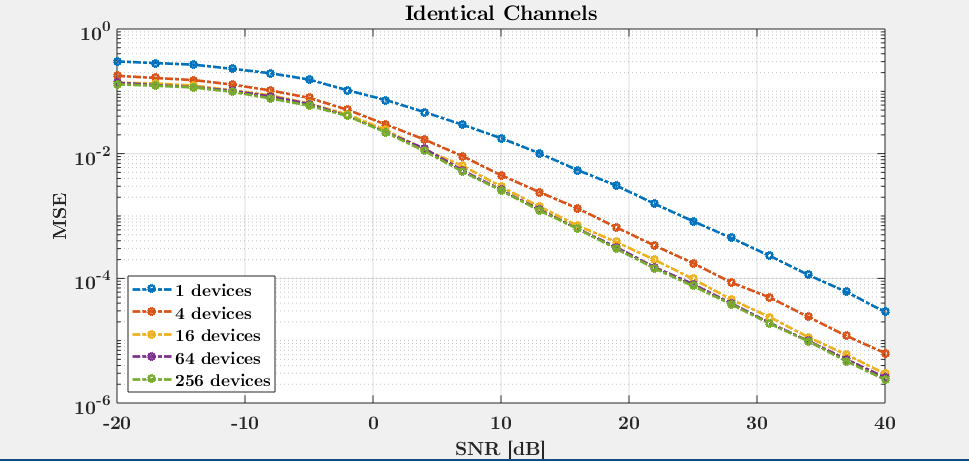
\includegraphics[
      width=12cm,
     height=14cm,
    keepaspectratio,]
    {users_change.png}
    \caption{Varying effect of the SNR vs MSE of different number of users in the network. This simulation has 4 re-transmissions and 4 subcarriers fixed. }
    \label{fig:effect_of_users}
\end{figure}

In \cref{fig:effect_of_users}, it can be seen that as we increase the number of users in the network, that the previous assumption of decreasing MSE would hold still. We can also see from Figure \ref{fig:effect_of_users} that the affect of increasing the users is beginning to saturate, slowing as we increase the number of users. This observation is also a sensible assumption, that as the number of users tends toward infinity, we would see more of a true likeness of the original distribution. 

% retransmissions
\textbf{Re-transmissions} \newline
Looking at the first of the two scenarios for re-transmissions, without power adaption, this situation does not take into consideration the power constrain described in \cref{sota}. It would be assumed that the effect of the increasing number of re transmissions would decrease the MSE, due to the averaging effect of re-transmitting the same information reducing the error in the estimate to the real distribution. 

\begin{figure}[H]
    \centering
    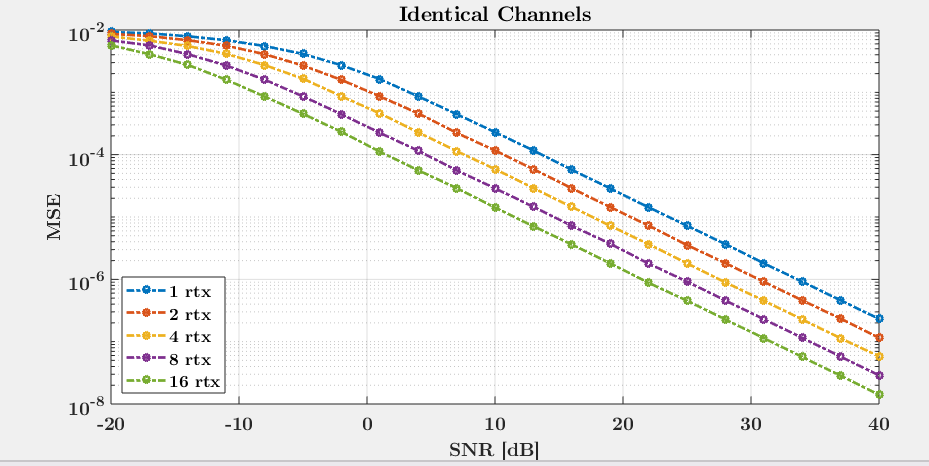
\includegraphics[
      width=12cm,
     height=14cm,
    keepaspectratio,]
    {retries_identical.png}
    \caption{Varying effect of the SNR vs MSE of different number of re-transmissions of the same channel. This simulation has 64 users and 16 subcarriers fixed.}    \label{fig:effect_of_retx}
\end{figure}

As per the previous assumptions, we can clearly see in Figure \ref{fig:effect_of_retx} increasing effect of the re-transmissions does indeed reduce the MSE of the system, however, this affect is only really seen at higher SNR ranges and the affect does seem to saturate quite quickly. This is due to the channel being deterministic, the effect of the re-transmission has less importance, as the noise $w$ is added after the summation of the signal at the fusion centre, thus there is nothing to average out from the received signal. This approach without taking into consideration this power constraint, would be a lot of overhead with respect to the amount of power needed

\textbf{Adaptive Power Re-transmissions} \newline
Lastly, looking at how the adapting the power across re transmissions affects the over all MSE. The idea is that such a system of TBMA should be constrained by power, it would be inefficient if every re-transmission and subcarrier index of the same signal was sent at full power, this would be a huge overhead for an information centric approach that utilises re-transmissions to increase the accuracy. Thus the idea was adopted such that each user would transmit their respective signal with power,$\frac{1}{L}$, where L is the total number of re-transmissions of the scheme. It would be expected that this approach would be similar to that of full power re-transmissions, where more re-transmissions result in decreased MSE. 

\begin{figure}[H]
    \centering
    \includegraphics[
      width=12cm,
     height=14cm,
    keepaspectratio,]
    % {event_subcarriers_change.png}
    {Adaptive_power_deterministic.png}
    \caption{Varying effect of the SNR vs MSE of having an adaptive power of each signal transmitted based on the number of retransmission.  }
    \label{fig:adapt_det_retx}
\end{figure}

Looking at Figure \ref{fig:adapt_det_retx}, we can see a similar downward trend in the MSE, however it would appear that using the adaptive power seems to decrease the performance as we increase the number of re-transmissions. This could be due to the deterministic channel and lack of random channel response to average out the transmitted signal. This could also be down to the fact that the noise would have more influence on the actual values being sent after the normalisation because with full power per transmission, the additional noise has less of an overall impact.


\subsubsection{Fading Channel}
Now, looking at the same scenarios, but using a random Gaussian complex channel. The same preconceived ideas should apply for all three use cases, however due to the more realistic channel, we should see more noisy representations of what the deterministic channel showed.

% users
\begin{figure}[H]
    \centering
    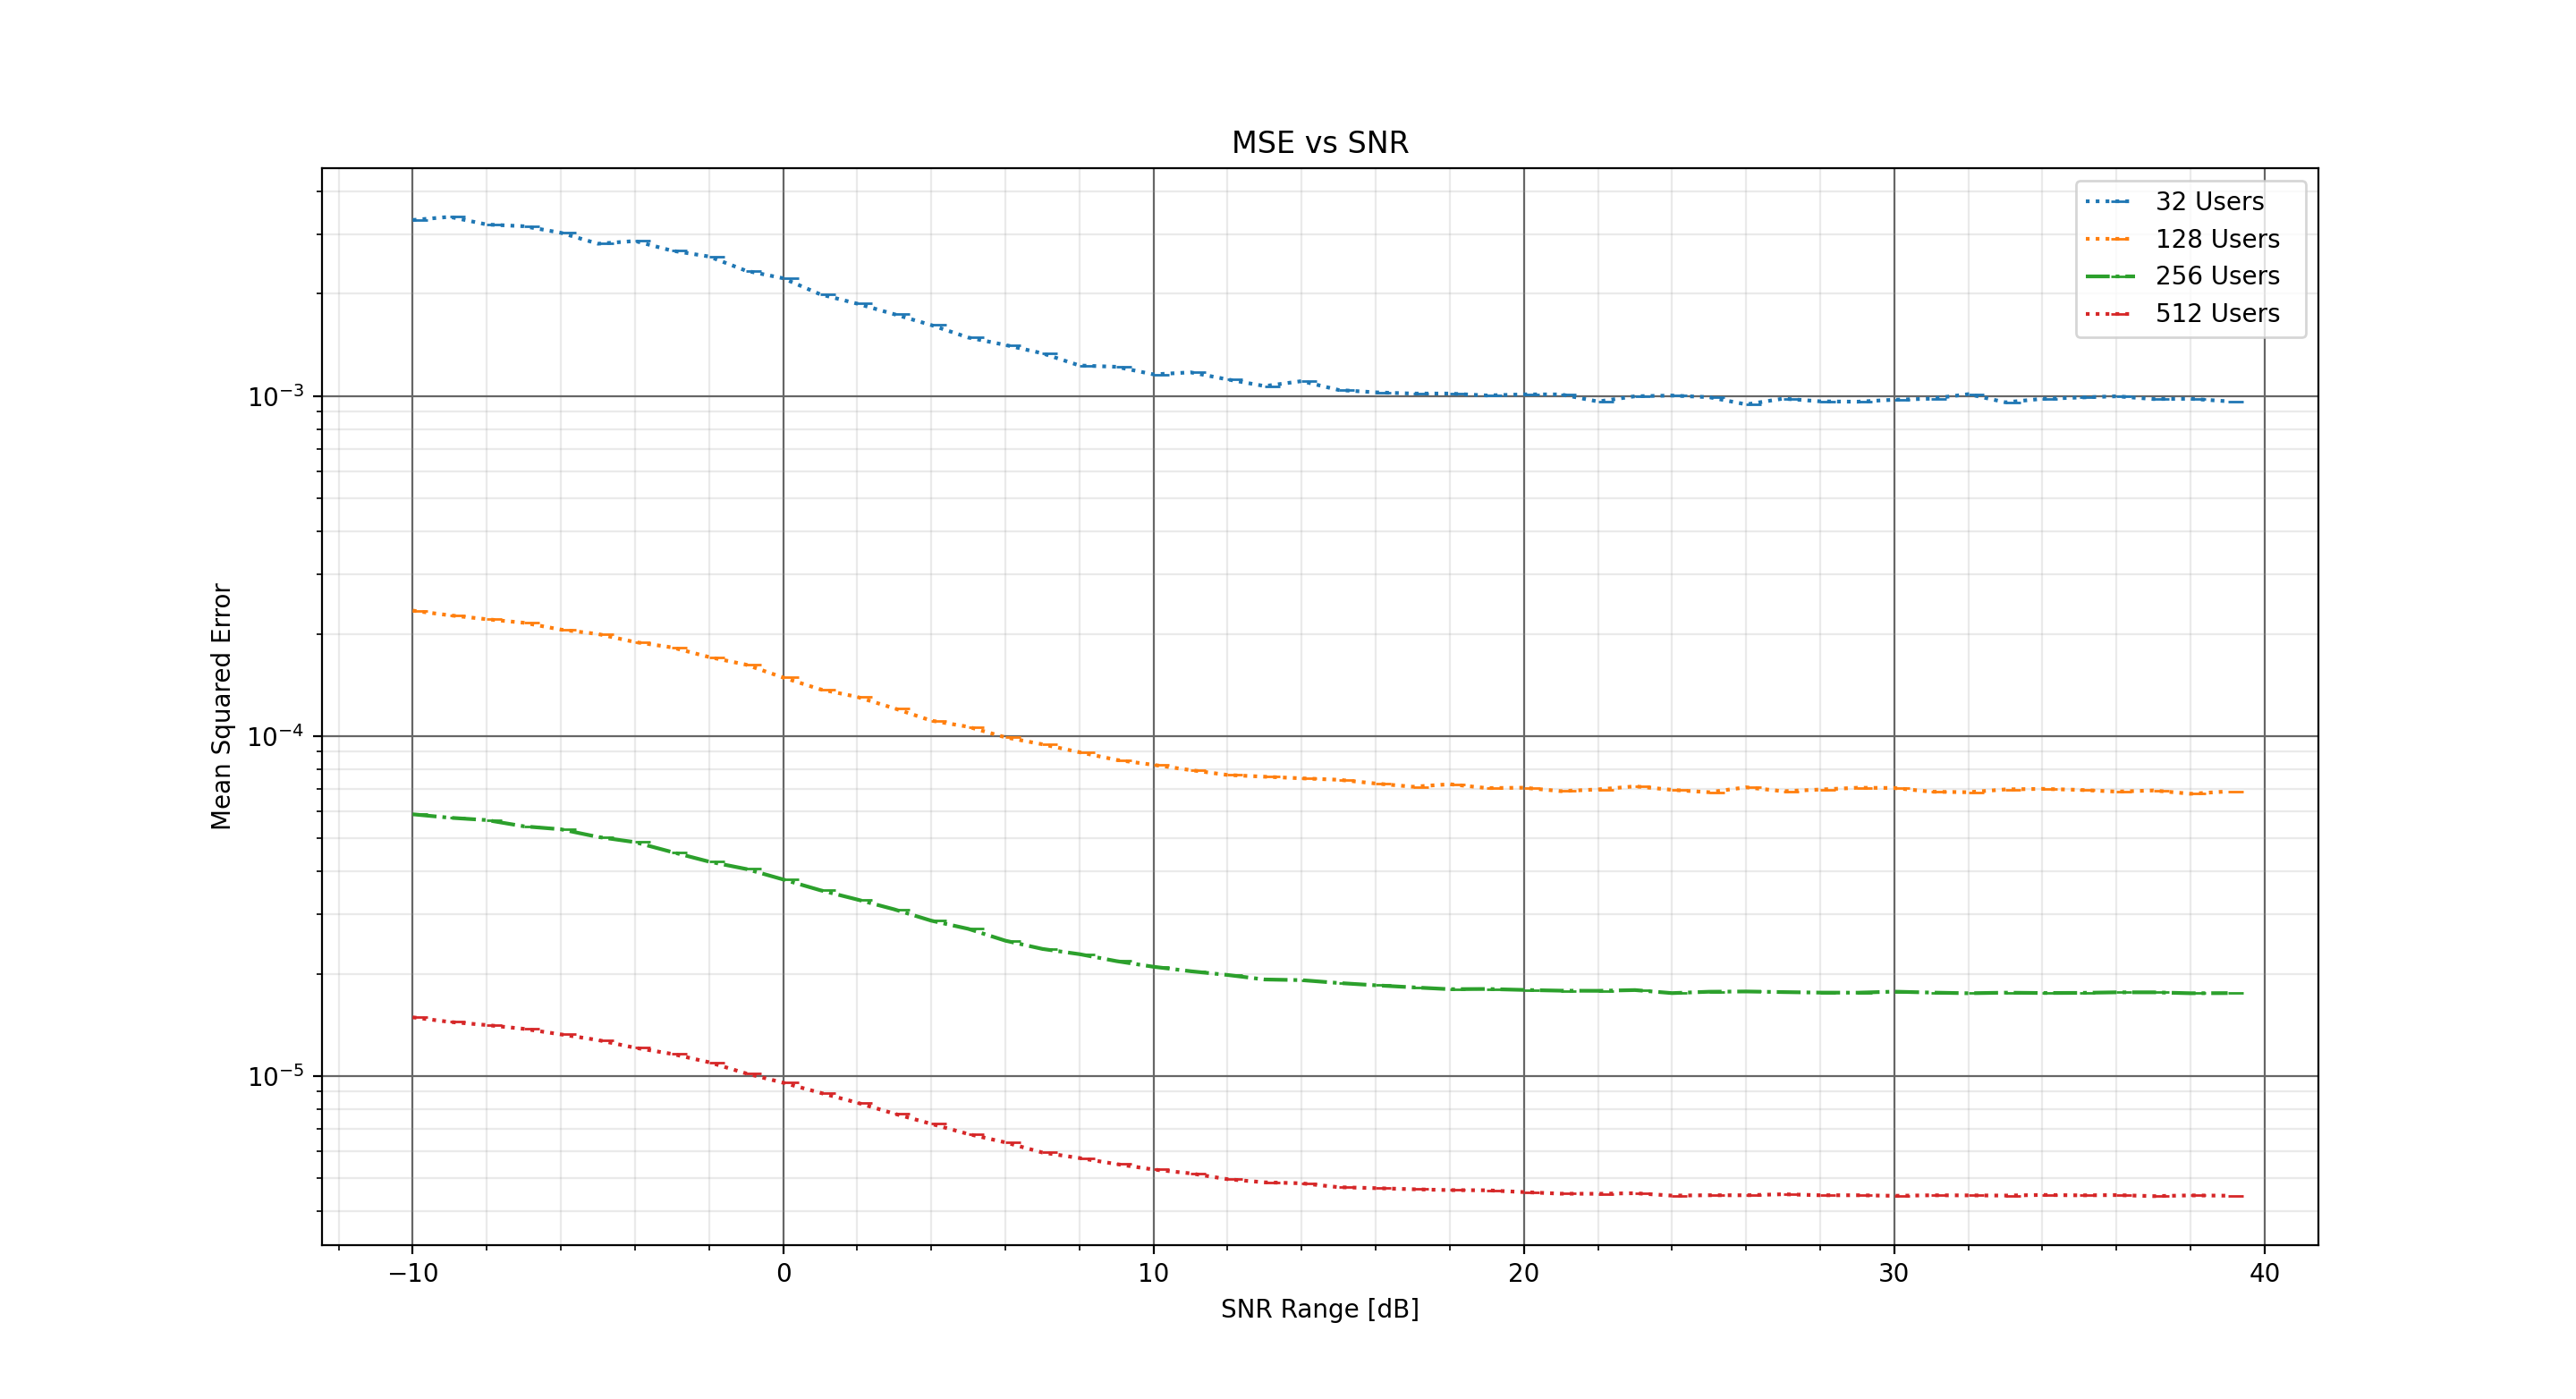
\includegraphics[
      width=12cm,
     height=14cm,
    keepaspectratio,]
    {users_randoms.png}
    \caption{Varying effect of the SNR vs MSE of different number of users in the network. This simulation has a 4:1 ratio of users to subcarriers. }
    \label{fig:effect_of_users_random}
\end{figure}

In Figure \ref{fig:effect_of_users_random}, it can be seen that even with a random complex channel that increasing the number of users still decreases the MSE, of course, the MSE is generally much higher in the random channel, thus we observe the initial MSE of the corresponding plots to be different. We also notice that the MSE seems to saturate around the 15dB mark. [To explain why this saturation is seen].

% retransmissions
\begin{figure}[h]
    \centering
    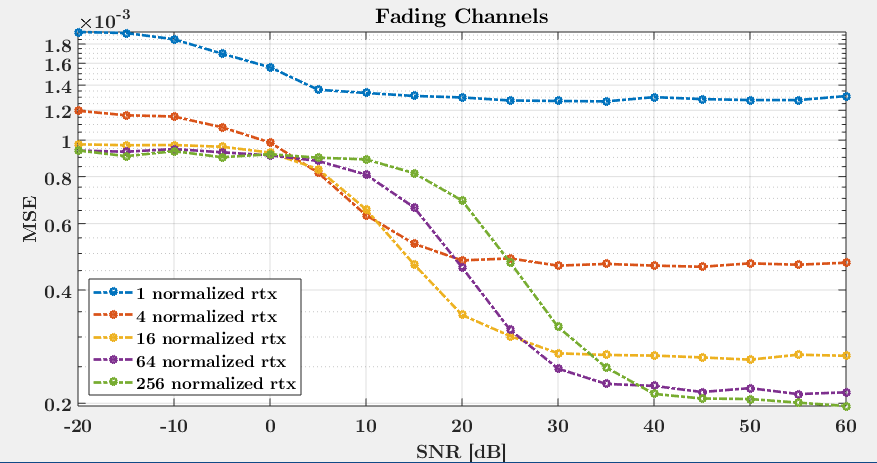
\includegraphics[
      width=12cm,
     height=14cm,
    keepaspectratio,]
    {fading_retries.png}
    \caption{Varying effect of the SNR vs MSE of different number of re-transmissions of the same channel. This simulation has 64 users and  1 subcarriers fixed.}    \label{fig:effect_of_retx_random}
\end{figure}


In Figure \ref{fig:effect_of_retx_random}, much like the non power adaptive approach in \ref{fig:adapt_det_retx}, the MSE is decreased overall with the increase of re-transmissions with saturation as the number increases. Again, we observe this initial sharp decrease in the MSE for low SNR values, then coming to a saturation point around 15-20dB. 


Lastly, looking at how the adapting the power across re transmissions affects the over all MSE. Figure \ref{fig:adapt_random_rtx} plot is comparable to Figure \ref{fig:adapt_det_retx}, however unlike Figure \ref{fig:adapt_det_retx}, we do not see this decrease in performance when we increase the number of re-transmissions $L$, conversely we see what was expected in the prior assumptions, that as we increase the number of re-transmissions the MSE decrease and the performance gain is noted. 

% \subsubsection{Different Schemes}
% Now we will look at the comparison of the different schemes which were presented in the Section \ref{schemas_and_channels}. The following numerical analysis of above proposed schemes have different distributions based on the scheme, where the environment has 64 Users, 16 subcarriers and 4 re-transmissions
% \begin{itemize}
%     \item Scheme \ref{fig:xor_schema} for the data model found in \ref{eq:event01common}, which splits the available subcarrier in half, half used for ACK and the other for NACK. The analysis at the start of each simulation takes a random number between the 0 and $K$ users which is then used to assign the number of ACKS for the simulation. The choice of encoded subcarriers is uniformly distributed across all available.
%     \item Scheme \ref{fig:cqi_ind} for the data model found in \ref{eq:event02independent}. This approach chooses a uniform random subcarrier to assign a value to, which equates to a real world CQI value. 
%     \item Scheme \ref{fig:cqi_pmf} for the data model found in \ref{eq:event03PMF}. Similarly to the previous approach, a random value is chosen for the CQI value, however this time the simulation takes a normally distributed sample of 1000 values which mean of the random value, this generated PMF is then transmitted along the channel. 
% \end{itemize}

% It would be expected that all of the schemes have similar MSE across a given SNR range with slight fluctuations depending on the respective encoding. However, it would be expected that channel schemes that are transmitting non correlated information could perform slightly worse as the resolution of the information increases, thus the error would probably increase too. Conversely, it would be a sound assumption that when the users in a group are transmitting common information, the MSE should be decreased. It would also be expected that underlying similarities are more prominent in the deterministic channel vs the random one. 


% Both the deterministic channel and the complex random channel have been compared, below in Figure \ref{fig:comp_mse_det}, we can see the results of the deterministic channel. As expected, the correlated information for  both CQI cases outperforms the ACK/NACK use case, which given the prior assumptions would make sense, as the ACK/NACK is transmitting mutually exclusive information, thus the assumption about correlation would not apply here. On the other hand, it can be seen that both CQI use cases perform similarly.

% \begin{figure}[H]
%     \centering
%     \includegraphics[
%       width=12cm,
%      height=14cm,
%     keepaspectratio,]
%     {comparison_det_3schemes.png}
%     \caption{MSE Vs SNR - comparison of different schemes, deterministic complex channel}
%     \label{fig:comp_mse_det}
% \end{figure}

% Looking now at the random complex channel analysis, seen in Figure \ref{fig:comp_mse_rand}, it can be seen that still the ACK/NACK scheme is still performing the worst. What is notable here, however is that in Figure \ref{fig:comp_mse_det}, the PMF and the Individual CQI scores perform similar. However, when the channel is random complex, we notice that the CQI PMF outperforms the individual CQI scheme. It can be said that is expected, due to the nature of each user transmitting correlated information in the form of a PMF, which has been seen in section \ref{case3}. 

% \begin{figure}[H]
%     \centering
%     \includegraphics[
%       width=12cm,
%      height=14cm,
%     keepaspectratio,]
%     {scheme_comp_16sc_64users_4rtx.png}
%     \caption{MSE Vs SNR - comparison of different schemes, random complex channel}
%     \label{fig:comp_mse_rand}
% \end{figure}

\subsection{srsLTE environment}
The evaluation and testing of the above proposed proof of concept method and implementation is evaluated and tested in this section, result are presented and discussed. Here, we take into consideration the two different approaches as per the simulation in previous sections. Initially we check the viability of the solution using a channel equal to 1, meaning an identical channel. Next, we move forward to verifying the approach with a random normal complex channel, with mean 0 and standard deviation 1. These two approaches were conducted for various random ACK/NACK combinations and varying UEs with adaptive power and fixed. 

\subsubsection{Identical Channel}
Several different tests were conducted with a deterministic channel to see if the ratio of ACKs to NACKs could be understood, this would be a great additional feature to the LTE, as for the reasons discussed earlier about redundancy and the more effective usage of the radio resources available for larger scale networks and users. 

Simulations of 10, 50 and 100 users were conducted, with a range of different of parameters for the retries and the various ACK/NACK combinations. This subsection only shows an overview as the channel is deterministic. This deterministic channel is used as a bench mark to ensure the encoding and decoding of the combined TBMA channel performs as expected. 

\begin{table}[H]
    \centering
 \begin{tabular}{||c c c c||} 
 \hline
 No. UEs & No. ACK/NACK & No. Retx & Result \\ [0.5ex] 
 \hline\hline
 10 & 0.3/0.7 & 10 &  0.3/0.7 \\ 
 \hline
 50 & 0.3/0.7 & 10 & 0.3/0.7 \\
 \hline
 100 & 0.6/0.4 & 30 & 0.6/0.4 \\
 \hline
 200 & 0.6/0.4 & 30 & 0.6/0.4 \\ [1ex] 
 \hline
\end{tabular}
    \caption{Results of deterministic channel srsLTE POC}
    \label{tab:my_label}
\end{table}

\subsubsection{Fading Channel}
The same setup and tests as above for the a random complex channel were also conducted, this random complex channel is modelled as $\mathcal{CN}(0,1)$. However, now as this channel is no longer deterministic, the below results are more specific and to the individual simulations conducted in the previous sections of this thesis. We will look at the results of the following situations:

\begin{enumerate}
    \item Increasing UEs, fixed re-transmissions, fixed ACK/NACK. 
    \item Increasing re-transmissions, fixed UEs, fixed ACK/NACK
    \item Varying ACK/NACK, fixed UEs, fixed re-transmissions.
\end{enumerate}

Situation 1, we would expect that the increasing number of UEs in the feedback TBMA , that the received and decoded ACK/NACKs would tend towards the real world values that had been transmitted. 

\begin{table}[H]
    \centering
 \begin{tabular}{||c c c c||} 
 \hline
 No. UEs & No. ACK/NACK & No. Retx & Result \\ [0.5ex] 
 \hline\hline
 10 & 0.7/0.3 & 10 &  0.086/0.913 \\ 
 \hline
 50 & 0.7/0.3 & 10 & 0.251/0.749 \\
 \hline
 100 & 0.7/0.3 & 10 & 0.399/0.601 \\
 \hline
 200 & 0.7/0.3 & 10 & 0.718/0.282 \\ [1ex] 
 \hline
\end{tabular}
    \caption{Results of random channel, Increasing UEs srsLTE POC}
    \label{tab:rand_chan_UEs_increase}
\end{table}

As expected we see in \cref{tab:rand_chan_UEs_increase}


Next we look at the varying affect of the re-transmissions on the received 

\begin{table}[H]
    \centering
 \begin{tabular}{||c c c c||} 
 \hline
 No. UEs & No. ACK/NACK & No. Retx & Result \\ [0.5ex] 
 \hline\hline
 200 & 0.3/0.7 & 10 &  0.699/0.301 \\ 
 \hline
 200 & 0.3/0.7 & 50 & 0.3/0.7 \\
 \hline
 200 & 0.6/0.4 & 100 & 0.6/0.4 \\
 \hline
 200 & 0.6/0.4 & 200 & 0.6/0.4 \\ [1ex] 
 \hline
\end{tabular}
    \caption{Results of random channel, varying ACK/NACKs srsLTE POC}
    \label{tab:rand_chan_rtx_increase}
\end{table}

As we can see from \cref{tab:rand_poc_res}, 

Finally for completeness, we look at the performance of the varying ACK/NACK combinations, we would assume that the combination of ACK/NACK being transmitted shouldn't make much of a difference, perhaps when All the UEs have a equal consensus on the outcome we would see slightly undesirable behaviour and when things are equal we may not 

\begin{table}[H]
    \centering
 \begin{tabular}{||c c c c||} 
 \hline
 No. UEs & No. ACK/NACK & No. Retx & Result \\ [0.5ex] 
 \hline\hline
 10 & 0.3/0.7 & 10 &  0.3/0.7 \\ 
 \hline
 50 & 0.3/0.7 & 10 & 0.3/0.7 \\
 \hline
 100 & 0.6/0.4 & 30 & 0.6/0.4 \\
 \hline
 200 & 0.6/0.4 & 30 & 0.6/0.4 \\ [1ex] 
 \hline
\end{tabular}
    \caption{Results of random channel, Increasing retransmissions srsLTE POC}
    \label{tab:rand_chan_rtx_increase}
\end{table}

\section{Summary and outlook}\label{summary_out}

This thesis has presented a goal orientated approach for multiple users to transmit correlated information across a wireless medium using type based multiple access. Firstly, in a simulation environment, looking into which attributes of the simulation play the biggest role into minimising the error. This led to identifying that the number of re-transmissions of the same data helped increase the accuracy of the TBMA channel. However, this led to an interesting idea that all nodes in a multicast group sending re-transmitted data at full power is both redundant and counter productive, so the power constraint that all transmissions for a TBMA channel, should not exceed the combined power limit of 1.

This simulation could be extended to take into consideration various other encoding schemes and spreading said schemes across multiple subcarriers to better the signal diversity and possible attain better results. Other evaluation metrics could be used apposed to that of the MSE, for example, KL divergence could be used in future to understand the divergence from the underlying PMF to the received one.  

Looking into how to apply this TBMA to real world LTE framework was the next step, looking closely how the like of ACK/NACK re transmission works in the current setup, was the introductions to knowing how TBMA in relation to ACK/NACK could be integrated into the likes of the current LTE network. Identifying how the simplest form of feedback worked in LTE led to a design choice around the PUCCH transmission of ACK/NACK through format 1A. Further investigation into how the the  mapping of these high level concepts of ACK/NACK to the physical resource was investigated. 

Upon understanding how these feedback channels works through 3GPP specification led into a proof of concept implementation through a LTE complaint open source SDR project called srsLTE, this project adheres to the same implementation found in the technical specifications from the 3GPP. Through the use of some stock test file which follows the normal LTE procedure for encoding and decoding up-link transmission, an adaption of the aforementioned test was created to allow for the encoding and decoding of 2 subcarrier TBMA channel with ACK/NACK in mind. Although this implementation was not strictly done over a radio interface, it was however propagated through all the respective functionality which it would be exposed to in normal LTE mode through the srsLTE project. In an attempted to ensure the most realistic representation of the setup without an actual radio interface, a modelled complex channel was introduced to bridge this gap. 

Overall as expected the result for the deterministic approach were always perfect representations of the ground truth. Although this is not a realistic situation, it has given the basic backbone for knowing that the process of encoding and decoding the TBMA channel was indeed plausible. Contrast to this, looking at the result when there was a complex random channel introduced between the encode/decode of the symbols, we can see that although exact ratios were not achieved. However, we see that the resultant ratios are still of within suitable range of error, and could be of use in the real world. 

Moving forward and next steps, would be to trial the same system over a physical radio link. Although the simulated channel is a good model of the real world, to ensure this would be a completely viable solution, it should be trialled with a real radio link. Upon verifying that this assumption is correct, next steps should be to implement the other encoding schemes as per the \cref{schemas_and_channels}. Extending the implementation from 2 fields for ACK/NACK to multiple fields capable of conveying more granular data would be a suitable next step. The current setup for encoding ACK/NACK would also need to be extended for encoding PMFs from the UEs, currently this POC only encompasses a one-shot style on one signature on the PUCCH. 

This thesis has only investigated how the TBMA approach could be integrated into the lower layers of the LTE network, more investigation into how the higher layers of the LTE stack would play a role in the formation and organisation of these TBMA packets. More over, other considerations to be taken into account moving forward would be such items as, testing the viability of integrating this approach with live ACK/NACK date from the unicast channel, how could this be multiplexed given the current setup in LTE. Other questions remain open too - should this TBMA have its own predefined format for the PUCCH or should it just utilise the remaining free areas in the PUCCH/PUSCH, what style of priority should be used. This proof of concept implementation merely address the physical how to of TBMA and does not take into consideration other related questions about how the finer integration should work.

\section{Glossary}\label{glossary}

\begin{align}
    L(\theta) = \prod_{i=1}^n\frac{2x_{i}}{\theta^2}e^{-\frac{x_{i}^2}{\theta^2}}
\end{align}
\begin{align}
    L(\theta) = \prod_{i=1}^n x_{i}(\frac{2}{\theta^2})^n e^{-\frac{\sum{x^2}}{\theta^2}}
\end{align}

Then taking the $ln$ log of both sides to simplify:

\begin{align}
    \ln{L(\theta)}= \ln{(x_{1},x_{2}\dots,x_{n})} + n\ln{2} - n\ln\theta^2 {-\frac{\sum{x^2}}{\theta^2}}\ln{e}
\end{align}
\begin{align}
    \ln{L(\theta)}= \sum\ln{x_{i}} \cdot + n\ln{2} - 2n\ln{\theta} -\frac{\sum{x^2}}{\theta^2}
\end{align}

Differentiating with respect to $\theta$, gives:

\begin{align}
    \frac{\partial }{\partial \theta}\ln L{(\theta)} = -2n\frac{\partial}{\partial\theta}\ln\theta - \sum x_{i}^2\frac{\partial}{\partial\theta}(\frac{1}{\theta^2})
\end{align}

\begin{align}
    \frac{\partial }{\partial \theta}\ln L{(\theta)} = -\frac{2n}{\theta} + \frac{2\sum x_{i}^2}{\theta^3} \dots \dots \dots
\end{align}

Now setting the partial derivative of $\theta$ equal to $0$ so we can get a maximum.

\begin{align}
    \frac{\partial }{\partial \theta}\ln L{(\theta)} = 0
\end{align}

\begin{align}
    -\frac{2n}{\theta} + \frac{2\sum x_{i}^2}{\theta^3} = 0
\end{align}
\begin{align}
    \frac{n}{\theta} = \frac{2\sum x_{i}^2}{\theta^3}
\end{align}
\begin{align}
   n\theta^2= \sum x_{i}^2
\end{align}

Thus we attain:

\begin{align}
    \theta^2 = \frac{\sum x_{i}^2}{n}
\end{align}


\addcontentsline{toc}{section}{References}
\bibliographystyle{plain}
\bibliography{\jobname}
\begin{thebibliography}{9}
\bibitem{3gpp36321}
3GPP TS 36.321 Medium Access Control (MAC) protocol specification, Release 15, 2020
\bibitem{3gpp38321}
3GPP TS 38.321 Medium Access Control (MAC) protocol specification, Release 15, 2020
\bibitem{ETSITS136213}
Evolved Universal Terrestrial Radio Access (E-UTRA), Physical layer procedures 
\bibitem{shannon_theory}
A Mathematical Theory of Communication, By C. E. SHANNON
\bibitem{information_centric}
Din, I.U., Asmat, H. and Guizani, M. A review of information centric network-based internet of things: communication architectures, design issues, and research opportunities. Multimed Tools Appl 78, 30241–30256 (2019). 
\bibitem{lte_advaned_mobile}
4G: LTE/LTE-Advanced for Mobile Broadband, Erik Dahlman, Stefan Parkvall, Johan Skold
\bibitem{tbma}
G. Mergen and L. Tong, "Type based Estimation over Multiaccess Channels" in IEEE 
\bibitem{access_tech}
Chen, W.K., "The Electrical Engineering Handbook", P.1005, Section 7.1 Access Technologies, 2004.
\bibitem{mod_impact}
Impact of Modulation Schemes on LTE, Juhi Pruthi, Pooja Agarwal, Nikita Jain.
\bibitem{umts_sesia}
LTE – The UMTS Long Term Evolution: From Theory to Practice Stefania Sesia, Issam Toufik and Matthew Baker.
\bibitem{csi_defs}
R\&STS8980 test system analyzes LTE quality indicators: CQI, PMI and RI
WIRELESS TECHNOLOGIES | Conformance test systems. 
\bibitem{fdma_info}
Chen, W.K., "The Electrical Engineering Handbook", P.1005, Section 7.1.1 FDMA, 2004. 
\bibitem{tdma_info}
Chen, W.K., "The Electrical Engineering Handbook", P.1006, Section 7.1.2 TDMA, 2004.
\bibitem{cdma_info}
Chen, W.K., "The Electrical Engineering Handbook", P.1007, Section 7.1.3 CDMA, 2004.
\bibitem{ofdma_info}
Sassan Ahmadi, LTE-Advanced,2014. Orthogonal Frequency Division Multiple Access. Section 9.5
\bibitem{srsLTE}
srsLTE opensource project, https://www.srslte.com/ 
\end{thebibliography}
\end{document}

